\documentclass[cn,11pt,twocol]{elegantbook}

\title{程序设计竞赛中的数论}
\subtitle{基础篇}

\author{陈昱翔}
\institute{AHU ACM-ICPC Lab}
\date{\today}
\version{1.0}

\extrainfo{Euclid marched into the wonderful world of Number Theory alone. --- Millay, 1923}

\logo{logo.png}
\cover{cover.jpg}

\usepackage{xcolor}


\colorlet{mygray}{black!30}
\colorlet{mygreen}{green!60!blue}
\colorlet{mymauve}{red!60!blue}

\lstdefinestyle{codestyle2}{
	backgroundcolor=\color{white},  
	basicstyle=\small\ttfamily,
	columns=fullflexible,
	breakatwhitespace=false,      
	breaklines=true,                
	captionpos=b,                    
	commentstyle=\color{mygreen}, 
	extendedchars=true,              
	frame=single,                   
	keepspaces=true,             
	keywordstyle=\color{blue},      
	language=c++,                 
	numbers=left,                
	numbersep=5pt,                   
	numberstyle=\small\color{blue}, 
	rulecolor=\color{mygray},        
	showspaces=false,
	showstringspaces=false,               
	showtabs=false,                 
	stepnumber=1,                  
	stringstyle=\color{mymauve},    
	tabsize=4,                 
	title=\lstname
}

\begin{document}
	
\maketitle

\tableofcontents


\mainmatter
\hypersetup{pageanchor=true}

\chapter*{写在前面}
\addcontentsline{toc}{chapter}{写在前面}
\markboth{Introduction}{}
	参加ACM-ICPC已经快三年了,想着留下些什么,于是决定将数论方面的一些知识整理成册,供后人参考。
	
	这本册子的目的是{\heiti 降低参赛同学们收集数论相关知识的时间成本},对知识点的介绍尽量做到详细且通俗易懂。
	书中会对所有出现的题目提供solution,一些经典的定理、结论还会提供证明。
	
	在册子完成过程中,AHU ICPC-Lab的同学们提出了许多宝贵意见,在此向他们表示衷心的感谢。此外,本书使用了ElegantBook模板
	(\href{https://github.com/ElegantLaTeX/}{https://github.com/ElegantLaTeX/}),减少了许多排版方面的工作,在此也表示感谢!
		
	由于本人水平所限,书中一定存在不少错误,欢迎同学们在GitHub上提出issues或者邮件联系我。\\
	
	\vbox{}
	

联系方式:
	\begin{itemize}
		\item GitHub 网址:\href{https://github.com/Feynman1999/number-theory-tutorial-in-Programming-Competition}{https://github.com/Feynman1999/number-theory-tutorial-in-Programming-Competition}
		\item 邮件:\email{chenyx.cs@gmail.com}
	\end{itemize}

\vbox{}

本书的Tex源码开源在GitHub,未经本人许可不可用于商业用途。\\

\vbox{}

\begin{flushright}
陈昱翔

2019年11月
\end{flushright}
	
\chapter{数的整除性}
\begin{introduction}[本章内容提要]
	\item 欧几里得算法
	\item 拓展欧几里得算法
\end{introduction}

\section{最小公倍数}
两个数a与b(不全为零)的最大公因数是整除它们两个的最大数,记为$gcd(a,b)$。如果$gcd(a,b)=1$,我们称$a$与$b$互质。

求两个数最大公因数的最有效的方法是{\heiti 欧几里得算法},其核心操作是辗转相除,先看一个例子。

\begin{example}
	欧几里得算法求gcd(28,93)的例子。
	
	第一步用93除以28得商为3,余数为7,记作下面式子:
	$$
		93 = 3*28 + 7
	$$
	第二步用上一步的除数作为新的被除数,上一步的余数作为新的除数,即:
	$$
		28 = 4*7 + 0
	$$
	发现此时余数为0,算法不再继续。欧几里得算法指出当得到余数0时,除数(上一步的余数)就是最初两个数的最大公因数。所以
	gcd(28,93) = 7。
\end{example}

\begin{theorem}{欧几里得算法}{label}
	要计算两个整数a与b的GCD,先令$r_{-1}=a$且$r_{0}=b$,然后计算相继的商和余数:$r_{i-1}=q_{i+1}*r_{i}+r_{i+1} \quad (i=0,1,2,...)$,
	直到某余数$r_{n+1}=0$,最后的非零余数$r_{n}$就是a与b的最大公因数。
\end{theorem}

\begin{proof}
	考虑一般情形,有
	\begin{align*}
	r_{-1} &= q_1*r_0 + r_1 \\
	r_0 &= q_2*r_1 + r_2 \\
	r_1 &= q_3 * r_2 + r_3 \\
	r_2 &= q_4 * r_3 + r_4 \\
 	&\cdot \cdot \cdot\\
	r_{n-3} &= q_{n-1}*r_{n-2} + r_{n-1} \\
	r_{n-2} &= q_{n} * r_{n-1} + {\color{red} r_n} \\
	r_{n-1} &= q_{n+1} * r_n + 0 \\
	\end{align*}
	欧几里得算法说,最后的$r_n$就是gcd,那么我们先证明$r_n$一定是$a(r_{-1})$和$b(r_0)$的因子。
	
	由最后一行知,$r_n$整除$r_{n-1}$,于是由倒数第二行知$r_n$整除$r_{n-2}$,依次类推,$r_n$整除$r_{0}$和$r_{-1}$。
	
	下面再证明$r_n$是$a$与$b$的{\heiti 最大}公因数。假设$d$是$a$与$b$的任意公因数,则由上面式子第一行知$d$整除$r_1$,
	于是由第二行知$d$整除$r_2$,依次类推,$d$整除$r_n$,即$r_n$是最大的公因数。
	
	最后,还要说明一定存在$r_{n+1}$为0,易知,每一次余数都是严格递减的,所以余数最后总能到0。那自然会问,要多少步呢?
	实际上,{\heiti 欧几里得算法的步数至多是$b$的位数的7倍}。
\end{proof}


\lstinputlisting[language=C++, style=codestyle2]{code01/gcd.cpp}

说到GCD,往往还会提到最小公倍数(LCM),有如下式子
\begin{align*}
lcm(a,b) * gcd(a,b) &=a*b \\
lcm(S/a, S/b) &= S/gcd(a, b)
\end{align*}


\section{线性方程定理}

已知两个整数a,b,现在我们观察由a的倍数加上b的倍数得到的所有可能整数,也就是说{\heiti 考察$ax+by$得到的所有整数},其中x,y可以是任何整数。

例如取$a=42$,$b=30$,随意列出一些x,y,会发现得到的数都可以被6整除。这其实很显然,因为42和30都能被6整除。更一般的,{\heiti 显然形如$ax+by$的每个数被$gcd(a,b)$整除},因为$gcd(a,b)$整除a与b。

接着问题又来了,$ax+by=gcd(a,b)$是否一定有整数解呢?答案是肯定的。证明是利用{\heiti 拓展欧几里得算法},不停的将余数用a和b表示,{\heiti 最后的gcd(a,b)一定可以用a,b表示}。也称欧几里得回代法。

\begin{example}
欧几里得回代法解$60x+22y=gcd(60,22)$

首先写出欧几里得算法计算gcd(60,22)的过程:
\begin{align*}
60=2 * 22+16 \\
22=1 * 16+6 \\
16=2 * 6+4 \\
6=1 * 4+2 \\
4=2 * 2+0
\end{align*}

这表明gcd=2。下面关键来了,我们想用a,b表示倒数第二行$6=1*4+2$的那个2,就从第一行表示a,b回代,如表\ref{tab:欧几里得回代法示例}:

\begin{table}[!htbp]
	\centering
	\caption{欧几里得回代法示例}
	\begin{tabular}{cccc}
		\toprule
		原式  && & 带入过程  \\
		\midrule
		$a=2*b+16$&&  & $16=a-2*b$ \\
		$b=1*16+6$&& & $6=b-1*16=-a+3b$ \\
		$16=2*6+4$&& &  $4=16-2*6=3a-8b$ \\
		$6=1*4+2$ && & $2=6-1*4=-4a+11b$ \\
		\bottomrule
	\end{tabular}%
	\label{tab:欧几里得回代法示例}
\end{table}%
	
于是得到$x=-4, \ y=11$。

\end{example}

{\heiti 这样一行行进行,将陆续得到形如最新余数=a的倍数+b的倍数的等式,最终得到非零余数gcd,就给出了方程的解。}

\begin{note}
$gcd(a,b)$是否是形如$ax+by$的最小正整数呢?是的。因为$gcd(a,b)<=min(a,b)$。
\end{note}

\vbox{}

既然一个线性方程$ax+by=gcd(a,b)$总有整数解$x,y$,下面的问题是{\heiti 如何表述线性方程的所有解}。

先考虑$gcd(a,b)=1$的情况(即a,b互质,其他情况可以转换为互质),假设$x_1,y_1$是方程$ax+by=1$的一个解。
通过$x_1$加上b的倍数和$y_1$减去a的相同倍数,可得到其他解。即对于任何整数$k$,我们得到新解$(x_{1}+kb,y_{1}-ka)$。(带入即可验证)

\begin{proof}
	$(x_{1}+kb,y_{1}-ka)$可以给出方程的{\heiti 所有}解。
	
	假设$(x_{1},y_{1})$与$(x_{2},y_{2})$是方程ax+by=1的两个解,即$ax_{1}+by_{1}=1$ 且$ ax_{2}+by_{2}=1$ ,我们用$y_{2}$乘以第一个方程,用$y_{1}$乘以第二个方程,再相减消去b,整理后得到$ax_{1}y_{2}-ax_{2}y_{1}=y_{2}-y_{1}$。
	类似的,用$x_{2}$乘以第一个方程,用$x_{1}$乘以第二个方程,再相减便得到$bx_{2}y_{1}-bx_{1}y_{2}=x_{2}-x_{1}$。
	令$k=x_{2}y_{1}-x_{1}y_{2}$,则得到$x_{2}=x_{1}+kb \ ,\  y_{2}=y_{1}-ka$。得证。
\end{proof}

\vbox{}

再考虑$gcd(a,b)>1$的情况,为简便,令$g=gcd(a,b)$,由前面“欧几里得回代法”知方程$ax+by=g$至少有一个解$(x_{1},y_{1})$。
{\heiti 而$g$整除$a,b$},故$(x_{1},y_{1})$是简单方程$\frac{a}{g}x+\frac{b}{g}y=1$的解。
于是由前面证明,通过式子$x_1+k*\frac{b}{g},\ y_1-k*\frac{a}{g}$改变$k$的值可得到其他解。这就完成了对方程ax+by=g解的描述,我们把它概括为下面定理。


\begin{theorem}{线性方程定理}{label}
设$a$与$b$是非零整数,$g=gcd(a,b)$。方程$ax+by=g$总是有一个整数解$(x_{1},y_{1})$(也称贝祖定理),
它可由前面叙述的欧几里得回带法得到。则方程的每一个解可由$(x_{1}+k*\frac{b}{g},y_{1}-k*\frac{a}{g})$得到,其中$k$可为任意整数。
\end{theorem}

\vbox{}

现在我们想怎么用代码实现上面说到的回代法。

如果用上面的思路,我们似乎需要事先知道欧几里得的结果,然后根据结果去算系数。
但是一般用计算机求解gcd,是递归算法,就是说我们需要逆推(上面过程的逆过程),这样才能写出递归代码。

假设当前我们要处理的是求出a 和 b的最大公约数,并要求出 x 和 y 使得 $a * x + b * y=g$。
而我们已经求出了下一个状态:b 和 a\%b 的最大公约数({\heiti 欧几里得算法核心,a=b,b=a\%b}),并且求出了一组$x_1$ 和$y_1$ 使得:$ b * x_1 + (a\%b) * y_1 = g$。
那么这两个相邻的状态之间存在一种关系可以求解,我们知道$a\%b = a - (a/b)*b$,那么较末状态(先开始递归计算的)有:

\begin{align*}
b * x_1 + (a\%b) * y_1 &= g\\
b*x_{1} + (a-(a/b)*b) * y_{1} &= g \\
b*x_{1} + a*y_{1}-(a/b)*b*y_{1} &=g\\
a*y_{1} + b*(x_{1}-a/b*y_{1})&= g
\end{align*}
对比较先的状态(后递归到的,需要求的),需要求一组 x 和 y 使得:$a*x + b*y = g$ ,比较对应项系数得到
\begin{align*}
x &= y_1\\
y &= x_1 - a/b * y_1 \\
\end{align*}


这就是递归的关键,我们把它称为{\heiti 拓展欧几里得算法}。之所以叫拓展,是因为它相比欧几里得算法多了一小点,但能解决模线性方程、逆元、同余方程等许多经典问题(后面会介绍)。

递归的终止条件为$b=0$,这时候$x=1,\ y=0,\ a = gcd$。

\lstinputlisting[language=C++, style=codestyle2]{code01/exgcd.cpp}

\vbox{}

\begin{problemset}
	\item 拓展欧几里得算法的时间复杂度是多少?
	\item \href{http://poj.org/problem?id=1061}{青蛙的约会}
	\item \href{https://ac.nowcoder.com/acm/contest/201/C}{Utawarerumono}
\end{problemset}











\chapter{素数}
\begin{introduction}[本章内容提要]
	\item 质因数分解
	\item 筛选素数
	\item 大区间问题
	\item 梅森素数
	\item 完全数
	\item 因数之和函数
\end{introduction}

\section{质因数分解}
\begin{definition}{素数}{prime}
	素数$p$是大于1且它的因数只有1和$p$的整数。
\end{definition}

\begin{property}
	\label{pro:prime}
	令p是素数,假设p整除乘积ab,则p整除a或p整除b(或者p既整除a也整除b)  
\end{property}

\begin{theorem}{无穷多素数定理}{label}
	存在无穷多个素数。
\end{theorem}

\begin{proof}
	证明的思路是,假设我们现在有一个素数表,只要说明如何利用这些素数找出新的不在表中的素数,这样迭代下去,就
表明必有无穷多个素数。设素数表一开始为$p_1,p_2,...,p_n$,令$A = p_1p_2...p_n + 1$,设$q$是某个整除$A$的素数,且设其是
最小的那个,那么$q$一定不在最初的素数表中,因为如果$q=p_i$,则$q$能整除1,显然错误。于是我们可以无限扩充素数表。
\end{proof}

\begin{theorem}{素数定理}{label}
	当x很大时,小于x的素数的个数近似等于$x/ln(x)$,即
	$$
	\lim_{x\to\infty} \frac{\pi(x)}{x/ln(x)}=1
	$$
	其中$\pi(x)$为素数计数函数,$\pi(x) = \#\{prime\ p:p\le x\}$。
\end{theorem}

\begin{theorem}{素数整除性质}{label}
假设素数p整除乘积$a_1a_2...a_r$ ,则p整除$a_1 \quad ,a_2 \quad , ...,\quad a_r$ 中至少一个因数。
\end{theorem}

\begin{proof}
	使用上面的\hyperref[pro:prime]{性质}可以方便的证明该定理。
\end{proof}

\vbox{}

下面将用{\heiti 素数整除性质}证明每个正整数可唯一分解成素数的乘积(算术基本定理)。

\begin{theorem}{算术基本定理}{suanshu}
	每个整数n>=2可唯一分解成素数乘积$n=p_1p_2...p_r$。
\end{theorem}

\begin{proof}
算术基本定理包含两个断言:

断言1:数n可以以某种方式分解成素数的乘积;

断言2:仅有一种这样的因数分解方式(因数重排除外);

- 对于断言1的证明用到归纳证明法 (当N+1是合数时,其必然可以分解成$N+1=n_1*n_2$,而前面已经归纳完毕,即$n1,\ n2$一定可以分解成素数,因此得证)。

- 对于断言2,可以由定理\ref{thm:suanshu}证得。
\end{proof}

\vbox{}

下面考虑如何进行质因数分解。

简单直接的方法是试除2,3,4,5,...分解n,但效率较低。
考虑一个整数n,如果n本身不是素数,则必有整除n的素数$p\leqslant \sqrt{n}$ 。于是我们可以遍历$2\sim \sqrt{n}$
进行试除,时间复杂度为$O(\sqrt{n})$。如果提前预处理出所有素数,则可每次只试除素数,时间复杂度为$O(\frac{\sqrt{n}}{ln \sqrt{n}})$

\lstinputlisting[language=C++, style=codestyle2]{code02/factor.cpp}

\section{区间素数筛}

这里区间素数筛指的是给定一个上限$n$,要求出区间$[1,n]$中所有的素数。如果采用直接遍历每个数并判断是不是素数的方法,时间复杂度为$O(n^{3\over2})$,若$n>10^6$,则
不能在$1s$的时间内求解。下面介绍的两种筛法,均使用“筛选”的思想,时间复杂度分别为$O(nlog(logn))$和$O(n)$,在比赛中经常使用。

\subsection{埃氏筛法}
考虑如果一个数$n$如果是合数(非素数),那么它一定有小于等于$\sqrt{n}$的质因子,也即$n$是这个质因子的倍数。那么我们可以从小到大($2\sim n$)依次遍历每个数,并存在一些标记记录每个数是否是合数,当遍历到某个数
时,如果当前数没有被标记为合数(就一定是素数了),就把当前数的所有倍数标记为合数。代码如下:

\lstinputlisting[language=C++, style=codestyle2]{code02/aishi.cpp}

\begin{remark}
	代码中有两个关键的地方:
\begin{itemize}
	\item 第10行,只有当是素数时,才进行筛选,因为使用合数筛是多余的(该合数的质因子已经筛过了);
	\item 第12行,从$i*i$开始筛,因为$(i-1)*i,\ (i-2)*i,\ ...\ 2*i$已经被筛过了。
\end{itemize}
\end{remark}

考虑埃氏筛法的时间复杂度,由于每次只考虑素数去筛,即为:
$$
	n\sum_{p\le n} \frac{1}{p}\ , \quad p \ is \ prime
$$
上式可近似认为是$O(nloglogn)$,感兴趣的可以阅读\href{http://www.wikiwand.com/en/Sieve_of_Eratosthenes#/Algorithm_complexity}{Sieve\_of\_Eratosthenes\#/Algorithm\_complexity} 

\vbox{}

观察埃氏筛法,是否有重复被筛去的合数呢?有的,就是一些质数的较大的公倍数,比如12,当i=2时(从4开始)会筛12;当i=3时(从9开始)还会筛12。

\subsection{欧拉线性筛法}

	欧拉筛的思想是{\heiti 保证每个合数都被其最小的质因子筛去},这样就不会像埃氏筛那样重复筛某个数。

	首先其还是筛选法,考虑用什么筛的:对于每个i,乘以小于i的每个素数,直到能整除就停止,这样能保证每个数只被筛去一次。
	
	这个整除停止很关键,假设没有这个break,就会有很多重复。
	
	比如$i=6$,取质数3,筛去了18;$i=9$,取质数2,也筛去了18。
	
	再比如$i=6$,取质数5,筛去了30;$i=10$,取质数3,筛去了30;$i=15$,取质数2,筛去了30。
	
	如果加上break,则筛去18的是9*2,筛去30的是15*2。为什么18不会被6*3筛去? 因为$6\%2=0$
	提前break了。即若有一个素数$p|i$,则我用i和后面更大的素数去筛选,不如用p和更大的i去筛选,
	这样保证了筛掉每个数的是其最小质因子。
	
	
\lstinputlisting[language=C++, style=codestyle2]{code02/euler.cpp}

由于每个数只会被筛去一次,时间复杂度是$O(n)$。

\subsection{区间数的最大、最小质因子}
上面介绍的埃氏筛法和欧拉筛法经过一点改动就可以用来求区间数的最大质因子和最小质因子。

对于区间最大质因子,稍微增加点埃氏筛的复杂度,从$2*i$而不是$i*i$开始筛:

\lstinputlisting[language=C++, style=codestyle2]{code02/maxprime.cpp}

对于区间最小质因子,只需修改欧拉筛中标记数组即可,时间复杂度不变:

\lstinputlisting[language=C++, style=codestyle2]{code02/minprime.cpp}


\section{区间质因数分解}
这里区间质因数分解指的是给定一个上限$n$,要求出区间$[1,n]$中所有数质因数分解的结果。
可以用埃氏法先求出所有数的所有质因子;或者使用欧拉法求出区间数的最小质因子再利用区间信息求解。
\subsection{埃氏法}
先$O(nlogn)$求出每个数的所有质因子,再$O(nlogn)$直接除求出质因子对应的指数:

\lstinputlisting[language=C++, style=codestyle2]{code02/interaishi.cpp}

\subsection{欧拉法}
先$O(n)$欧拉筛求出每个数的{\heiti 最小质因子},再$O(nlogn)$利用区间信息求出对应的指数。
区间信息指的是,对于每个数如果我们都知道其最小质因子,则可以先将当前数的最小质因子除完,剩下的数的最小质因子我们还是知道的,于是继续除,直到1为止。
\lstinputlisting[language=C++, style=codestyle2]{code02/intereuler.cpp}

\section{大区间素数筛与质因数分解}
大区间指的是咱们考虑的区间不再是$[1,n]$,而是$[L,R]$,这里$R\le 2^{40}, \  R-L<=10^6$。

\subsection{大区间素数筛}
对于一个合数$n$,一定有小于等于$\sqrt{n}$的质因子,利用这一点,我们依然可以使用埃氏筛的思想。
先预处理出$[1,\sqrt{R}]$区间内的所有素数,然后拿这些素数去做筛选即可。

时间复杂度为$O(N + llogl)$ , 其中$N$为$\sqrt{R}$,$R$是区间右端点,即需要预处理的素数范围 ; $l$为区间长度$R-L$。

\lstinputlisting[language=C++, style=codestyle2]{code02/large-inter-prime.cpp}

\subsection{大区间质因数分解}
和上面类似,先埃筛求出小于等于$\sqrt{R}$的所有质因子,然后对于区间内的每个数直接除即可。

因为一个合数n大于$\sqrt{n}$ 的质因子最多只有1个,因此将已知的质因子全部除尽后,若不为1,就为那个大于$\sqrt{n}$的质因子,对应指数为1。

时间复杂度为$O(N + llogl)$,其中$N$为$\sqrt{R}$,$R$是区间右端点,即需要预处理的素数范围 ; $l$为区间长度$R-L$。

\lstinputlisting[language=C++, style=codestyle2]{code02/large-inter-factor.cpp}


\section{梅森素数与完全数}
梅森素数与完全数在程序设计竞赛中不是很常见,这里简要介绍一下。

\subsection{梅森素数}
现在我们来研究形如$a^n-1(n\ge2)$的素数。例如31就是这样的数,因为$31 = 2^5 - 1$。
由于$a-1$始终是$a^n-1$的因子。为啥呢?因为使用几何级求和公式:(展开即可证明该公式)
$$
x^n-1=(x-1)(x^{n-1}+x^{n-2}+...+x^2+x+1)
$$
所以若$a^n-1$为素数,则a一定等于2。反之显然不成立。

再进一步考虑$n$,假设$n$为合数,即$n=mk$,则$2^n=2^{mk}=(2^m)^k$。使用$x=2^m$的几何级数公式得:
$$
2^n - 1 = (2^m)^k - 1 = (2^m-1)((2^m)^{k-1}+(2^m)^{k-2}+...+(2^m)^2+(2^m)+1)
$$
这证明了若$n$是合数,则$2^n-1$也是合数。综上有以下命题:

\begin{proposition}{}{label}
	如果对整数$a\ge2$与$n\ge2$,$a^n-1$是素数,则$a$必等于2且$n$一定是素数。
\end{proposition}

形如$2^p-1$的素数叫做{\heiti 梅森素数},已知的梅森素数在\href{https://www.mersenne.org/primes/}{https://www.mersenne.org/primes/}中可以找到,
目前已经找到了51个(截至2019.09.03)。发现更多的梅森素数没有太大的数学意义,数学上更令人感兴趣的是下面的问题,其答案尚未知晓:

\begin{custom}{问题}
	存在无穷多个梅森素数吗?
\end{custom}

\subsection{完全数}

\begin{definition}{完全数}{wanquanshu}
	完全数是等于其真因数之和的数。真因数指的是小于自己的因数(即除去自己)。
\end{definition}


\begin{theorem}{欧几里得完全数公式}{label}
	如果$2^p-1$是素数,则$2^{p-1}(2^p-1)$是完全数。
\end{theorem}

\begin{proof}
	将$2^{p-1}(2^p-1)$所有真因数直接写出求和即证。
\end{proof}

这里的$(2^p-1)$不就是梅森素数吗?也就是说只要求得一个梅森素数,就得到一个完全数。

那欧几里得完全数公式是否表示了所有完全数呢?千年之后的欧拉证明了欧几里得完全数公式至少给出了所有{\heiti 偶完全数},称为欧拉完全数定理。

在介绍和证明欧拉完全数定理之前,我们先来介绍一个函数$\sigma(n)$。

\begin{center}
	$\sigma(n) = n$的所有因数之和(包括1和n)。
\end{center}

例如$\sigma(6) = 1 + 2+3+6 = 12$。下面试着写出其一般公式,$\sigma(p) = p+1$,$\sigma(p^k) = 1 + p+p^2+...+p^k = \frac{p^{k+1}-1}{p-1}$。

如果你用程序打个表,也许会发现$\sigma(mn)$时常会等于$\sigma(m)\sigma(n)$,实际上这在$m$和$n$互质时成立。

\begin{theorem}{$\sigma$函数公式}{label}
	\begin{itemize}
		\item 如果$p$是素数,$k\ge1$,则$\sigma(p^k) = 1 + p+p^2+...+p^k = \frac{p^{k+1}-1}{p-1}$;
		\item 如果$gcd(m,n)=1$,则$\sigma(mn) = \sigma(m)\sigma(n)$。
	\end{itemize} 
\end{theorem}

$\sigma$函数在程序设计竞赛中也时常出现(或者其类似函数,如因子个数函数),后面章节还会说到它,现在我们用它来辅助证明欧拉完全数定理。

显然,$\sigma$函数可以和完全数产生联系,如果$\sigma(n)=2n$,则n恰好是完全数。

\begin{theorem}{欧拉完全数定理}{label}
如果n是偶完全数,则$n$一定是$2^{p-1}(2^p-1)$ 的形式,其中$2^p-1$是梅森素数。
\end{theorem}

\begin{proof}
	假设n是偶完全数,n是偶数则说明可将它分解成$n=2^km,\quad k\ge 1 \ \&\ m\ is\ odd$
	
	则$\sigma(n)=\sigma(2^km)=\sigma(2^k)\sigma(m)=(2^{k+1}-1)\sigma(m)$。
	又n是完全数,则$\sigma(n)=2n=2^{k+1}m$。
	
	因此可以得到
	$$
	2^{k+1}m=(2^{k+1}-1)\sigma(m)
	$$
	由上式可知,由于$(2^{k+1}-1)$一定是奇数,所以$2^{k+1}| \sigma(m)$ ,于是设$\sigma(m)=c*2^{k+1}$ ,带入上式有:
	\begin{align*}
	2^{k+1}m=(2^{k+1}-1)*c*2^{k+1} \\
	m=(2^{k+1}-1)*c
	\end{align*}
	现在我们有两个式子,$m=(2^{k+1}-1)*c$ 和$\sigma(m)=c*2^{k+1}$。
	
	实际上这里c只能等于1,下面我们来证明$c=1$。
	
	假设$c>1$,则$m=(2^{k+1}-1)*c$至少被不同的数$1,c,m$所整除,因此有
	$$
	\sigma(m)\ge 1+c+m=1+c+(2^{k+1}-1)*c
	$$
	显然,这是错误的(会得出$0\ge 1$),因此$c=1$,所以$m=2^{k+1}-1$  ,  $\sigma(m)=2^{k+1}=m+1$,所以m是素数。
	
	现在我们已经证明了,如果n是偶完全数,则
	$$
	n=2^k(2^{k+1}-1)\ ,\quad where \ (2^{k+1}-1)\ is \ prime
	$$
	由于$2^{k+1}-1$是素数,则$(k+1)$一定是素数,(上节已说明)。令$k+1=p$,则$n=2^{p-1}(2^p-1)$,其中$2^p-1$是梅森素数。
	
	欧拉完全数定理证毕。
\end{proof}

\vbox{}

\begin{note}
	关于完全数的几个结论:
	\begin{itemize}
		\item 目前还没找到奇完全数
		\item 每个完全数的全部因数倒数之和都是2
		\item 除了6以外的完全数,每个都可以表示成连续奇数的立方和
		\item 每个完全数都可以表示成2的一些连续正整数次幂之和
		\item 完全数都是以6、8结尾
	\end{itemize}
\end{note}

\vbox{}

\begin{custom}{问题}
	存在奇完全数吗?
\end{custom}

\vbox{}

\vbox{}


\begin{problemset}
	\item 区间数的最大质因子是否有线性时间的算法?
	\item 大区间数的最小质因子是否有线性时间的算法?
	\item 试着写出求单点$\sigma(n)$以及区间$[1,n]$所有$\sigma$值的代码。
\end{problemset}
\chapter{同余}

\begin{introduction}
\item 同余方程
\item 快速乘、快速幂
\item 逆元、线性求区间逆元
\item 中国剩余定理
\item 欧拉降幂
\item 卡米歇尔数
\item Miller\_Rabin
\item Pollard\_Rho
\item 离散对数
\item 原根
\end{introduction}


\section{同余式与同余方程}
\subsection{同余式}
整除性是很好的性质,这在最大公因数、模线性方程和素数分解中均得到了体现。而同余式提供了一种
描述整除性质的简便方式。

\begin{definition}{同余}{label}
	如果$m|(a-b)$,我们就说a与b模m同余并记之为$a\equiv b(mod\ m)$。
	
	特别地,$a\equiv a\%m(mod\ m)$ 。
\end{definition}

数m叫做同余式的模。 具有相同模的同余式在许多方面表现得很像通常的等式。例如:

若$a_1\equiv b_1(mod\ m) \ ,\quad a_2\equiv b_2(mod\ m)$     则$a_1\pm a_2\equiv b_1\pm b_2(mod \ m)$ ,$a_1a_2\equiv b_1b_2(mod \ m)$ 

{\heiti 但 $ac\equiv bc(mod \ m)$ 时,未必有$a\equiv b(mod \ m)$,只有$gcd(c,m)=1$,才可以消去c。}


\subsection{同余方程}
如果同余式含有未知数,我们考虑如何求解。

首先考虑“穷举法” ,要解模m同余式,可让每个变量试取0,1,2...,m-1。例如,解同余式$x^2+2x-1\equiv 0(mod\ 7)$,
就去试$x=0\quad, x=1\quad,...\quad,x=6$,这样可以求出两个解$x\equiv 2(mod\ 7)$和$x\equiv 3(mod\ 7)$ 当然还有其他解,但新的解与2或3是同余的,如9和10。当我们说“求同余式的所有解时”,是指求所有不同余的解,即相互不同余的所有解。

许多同余式是没有解的,如$x^2\equiv 3(mod\ 10)$。

\vbox{}

下面考虑如何求解同余式$ax\equiv c(mod\ m)$。 
\begin{example}
解同余式$18x\equiv8(mod\ 22)$
\end{example}

等价于求$22\ |\ (18x-8)$,即求$18x-22y=8$。       

解这类方程的问题在第一章中研究过。

对于$ax\equiv c(mod\ m)$ ,其有解{\heiti 当且仅当}线性方程$ax-my=c$ 有解。


由前可知,线性方程$ax-my=c$ 有解的充分必要条件是$gcd(a,m)\ |\ c$。

且方程$au+mv=g$ 一定有解 ,设一个解为$(u_0,v_0)$,则有
$$
a\frac{cu_0}{g}+m\frac{cv_0}{g}=c
$$
这说明$x_0= \frac{cu_0}{g}$是同余式$ax\equiv c(mod\ m)$ 的一个解,通解为$x=x_0+k\cdot \frac{m}{g}$。

{\heiti 由于相差m的倍数的任何两个解认为是相同的},所有恰好有$g$个不同的解,这些解通过取$k=0,1,2...,g-1$而得到。将上述过程概述为定理:


\begin{theorem}{线性同余式定理$ax\equiv c(mod\ m)$}{label}
设a,c与m是整数,m>=1,且设$g=gcd(a,m)$。 

(a)  如果$g\nmid c$,则同余式$ax\equiv c(mod\ m)$ 没有解

(b)  如果$g\ |\ c$ ,则同余式$ax\equiv c(mod\ m)$ 恰好有g个不同的解。要求这些解,首先求线性方程$au+mv=g$ 的一个解$(u_0,v_0)$ 
{\heiti (欧几里得回带法,在计算机上递归求得,称为扩展欧几里得算法)} 。则$x_0=(\frac{cu_0}{g}\% \frac{m}{g} + \frac{m}{g}) \% \frac{m}{g}$是$ax\equiv c(mod\ m)$ 的解,不同余解的完全集由
$$
x\equiv x_0+k\cdot \frac{m}{g} \  (mod\ m),\quad k=0,1,2,...,g-1
$$
给出。
\end{theorem}


例如,同余式$943x\equiv 381(mod\ 2576)$ 无解,这是因为$gcd(943,2576) \nmid 381$。

另一方面,同余式$893x\equiv 266(mod\ 2432) $
有19个解,因为$gcd(893,2432)=19,\  19|266$     这个19即为不同余解的个数。

下面解方程$893u-2432v=19$ ,使用欧几里得回带法可以求得解$(u,v)=(79,29)$ ,乘以266/19=14得方程$893x-2432y=266$的解$(x,y)=(1106,406)$ ,
即1106是同余式方程的一个解,这样的互不同余的解共有19个。1106加上2432/19=128的倍数(\%2432)就可得到完全解集。


\begin{remark}
	线性同余式定理最重要的情形是$gcd(a,m)=1$ ,在这种情形下,同余式恰好有一个解。
\end{remark}

\lstinputlisting[language=C++, style=codestyle2]{code03/modequation.cpp}

\vbox{}

对于非线性的同余式,其解“不是很确定”。

我们熟悉的是对于{\heiti 一个d次实系数多项式的实根不超过d个} ,这个结论对于同余式并不成立。

例如$x^2+x\equiv 0(mod\ 6)$ 有4个模6不同的根:0,2,3,5。

但是,{\heiti 当p为素数时,这个结论依然成立:}

\begin{theorem}{模p多项式根定理}{label}
设p为素数,$f(x)=a_0x^d+a_1x^{d-1}+...+a_d$ 是次数为d>=1的整系数多项式,且p不整除$a_0$ ,则同余式$f(x)\equiv 0(mod\ p)$ 最多有d个模p不同余的解。
\end{theorem}

\section{快速乘与快速幂}
快速乘和快速幂作为工具经常在程序设计竞赛中遇见。
\subsection{快速乘}
在$C++$中,变量最多只能表示到$2^{64}-1$这么大,所以如果我们要计算$a*b\%c$,而$a,b$都是接近表示上限的数,这个时候就需要快速乘。
即将$b$按二进制位分解分别加上,时间复杂度为$O(log(b))$。
\lstinputlisting[language=C++, style=codestyle2]{code03/fastmul.cpp}

\subsection{$O(1)$快速乘}
上面的“快速乘”时间是$O(logb)$的,如果是两个63位数相乘(结果long long 存不下),则还有一个巧妙的方法可以简单解决这个问题:

\lstinputlisting[language=C++, style=codestyle2]{code03/o1fastmul.cpp}

首先使用浮点运算来得到$\left\lfloor\frac{a * b}{P}\right\rfloor$的值,显然$a*b-d*p$中的两个乘法都有可能会溢出,但是没关系,因为可以知道其差是一个64bit可容纳的正整数,那么溢出部分的差仅可能为0或者1,最后
特判处理一下即可。	
\begin{note}
	当然,如果编译器支持$int128$的话,可以直接用128位数。
\end{note}

\subsection{快速幂}
现在我们要计算$a^b\%c$,如果乘$b$次,时间复杂度太高,考虑将$b$按照二进制分解,每一位分别计算并乘在一起即可。
时间复杂度为$O(log(b))$。相比于快速乘,只是加法变了乘法。
\lstinputlisting[language=C++, style=codestyle2]{code03/fastexp.cpp}


\section{费马小定理与逆元}
前面我们讨论了关于同余式、同余方程的一些性质,小结一下,互质这个条件很重要。

\begin{itemize}
	\item 对于$ac\equiv bc(mod \ m)$,如果$gcd(c,m)=1$,则可以消去c,得到$a\equiv b(mod \ m)$ 。
	\item 对于同余方程 $ax\equiv c(mod\ m)$,若$gcd(a,m)=1$ ,同余式恰好有一个解。
\end{itemize}

{\heiti 对于式子$ax\equiv c(mod\ m)$,令$c=1$,得$ax\equiv 1(mod\ m)$,若$gcd(a,m)=1$,则方程有唯一解$x_0$,
我们称$x_0$为$a$在模$m$意义下的逆元,常记作$a^{-1}$。}

逆元可以用来说明一些事情,比如如果$ac\equiv bc(mod\ m)$,若$gcd(c,m)=1$,
则存在$c^{-1}$使得$cc^{-1}\equiv 1 (mod\ m)$。所以可以对$ac\equiv bc(mod\ m)$两边同时乘以$c^{-1}$,得到$a\equiv b(mod\ m)$。

如何求解逆元呢?拓展欧几里得即可,因为就是一个同余方程:
\lstinputlisting[language=C++, style=codestyle2]{code03/inverse.cpp}

\vbox{}

若模数是素数,我们还可以用费马小定理求解。

\begin{theorem}{费马小定理}{femat}
	设p是素数,a是任意整数且$p\nmid a$ ,则 $a^{p-1}\equiv 1(mod\ p)$。 
\end{theorem}

在证明费马小定理之前,先来看一个引理。

\begin{lemma}{为证明费马小定理做准备}{forfemat}
	设$p$是素数,a是任何整数且 $p\nmid a$ 则数
	$$
	a,2a,3a,...,(p-1)a\qquad (modp)
	$$
	与数
	$$
	1,2,3,...,(p-1)\qquad (modp)
	$$
	相同,尽管它们的次序不同。
\end{lemma}

\begin{proof}
	数列$a,2a,3a,...,(p-1)a$,包含$p-1$个数,显然没有一个数被$p$整除 ,假设从中取出两个数ja和ka是关于p同余的,即$p|(j-k)a$,
	又p是素数且p不整除a,所以p整除$(j-k)$。但是$|j-k|<p-1 $,所以$j-k=0$,即$j=k$。
	
	这表明,这p-1个数模p不同,由于任何数mod p仅有$p-1$个不同的非零值,证毕。
\end{proof}

\begin{proof}
	费马小定理的证明。
	
	利用该引理\ref{lem:forfemat},即可完成对费马小定理\ref{thm:femat}的证明,将上面引理列到的两组数相乘,可得到
	$$
	a^{p-1} \cdot (p-1)!\equiv (p-1)!   \qquad (modp)
	$$
	由于$(p-1)!$与p互质(显然除了1没有其它公共因子了),可以消去它(本节开头有提到这个性质),则$a^{p-1}\equiv 1(mod\ p)$。
\end{proof}

\vbox{}

有了费马小定理,若模数$m$是质数,则数$a$关于$m$的逆元就是$a^{m-2}$,因为$a* a^{m-2} \equiv 1 \ (mod p)$。
使用快速幂直接计算即可。

\vbox{}

{\heiti 使用费马小定理还可以进行素数测试},后面小节会提到。

\section{中国剩余定理}

\begin{theorem}{中国剩余定理}{CRT}
	设m与n是整数,$gcd(m,n)=1$,b与c是任意整数,则同余式组
	$x\equiv b(mod\ m)$与$x\equiv c(mod\ n)$恰有一个解$0\leqslant x<mn$。
\end{theorem}

\begin{proof}
	对于第一个同余式$x\equiv b(mod\ m)$,其解由形如$x = my +b$的所有数组成。将其带入第二个方程可得
	$my\equiv c-b (mod\ n)$,已知$gcd(m,n)=1$,由线性同余式定理知其恰有一个解$y_1,\ 0\le y_1<n$,则$x_1=my_1+b$
	给出了原来同余式组的解,这是在$[0,mn)$之间的唯一解。
\end{proof}

\vbox{}

上面只考虑了两个同余式,如果有多个呢?

\begin{custom}{问题}
	求出方程组$x\equiv a_i(mod \ m_i) (0 \leqslant i <n) $ 的解$x$,其中$m_0,m_1,m_2,m_3,...,m_{n-1}$ 两两互质。
\end{custom}

\begin{solution}
	令$M_i=\prod_{j\neq i}m_j$     则有$(M_i,m_i)=1$   
	
	故存在$p_i,q_i$ ,使得$M_i*p_i+m_i*q_i=1$ 
	
	令  $e_i=M_ip_i$,\quad    $p_i$即为$M_i$ 模$m_i$下的逆元。   
	
	则有
$$
e_i\equiv\left\{\begin{matrix}
0(mod\ m_j)\ ,\ j\neq i\\ 
1(mod\ m_j)\ ,\ j=i
\end{matrix}\right.	
$$	
	故$e_0a_0+e_1a_1+e_2a_2+...+e_{n-1}a_{n-1}$是方程的一个解。
	
	由中国剩余定理知,$[0\sim\prod_{i=0}^{n-1}m_i\}$ 中必有一解,将上式模$\prod_{i=0}^{n-1}m_i$即可。 
\end{solution}

时间复杂度  $O(nlogm)$,其中$n$表示有$n$个方程。

\lstinputlisting[language=C++, style=codestyle2]{code03/crt.cpp}

\begin{custom}{问题}
	如果这些方程的{\heiti 模数不互质}呢?(上面互质的方法只是一种巧妙的构造)
\end{custom}

一样可以求解,每一次我们将两个方程合并为一个方程,具体来说,假设目前的前两个方程为$x\equiv a_1 \ (mod\ m_1),\quad  x\equiv a_2 \ (mod\ m_2)$。
将第一个带入第二个可得到$km_1\equiv a_2-a_1 \ (mod\ m_2)$,解这个同余方程,求出$k$的最小正整数解$k_0$,那么$k = \frac{m_2}{gcd}y+ k_0$,带入
$x=km_1+a_1$中可以得到$x=\frac{m_1m_2}{gcd}y+m_1k_0+a_1$,也即将前两个方程合并为了一个:$x\equiv m_1k_0+a_1\ (mod\ \frac{m_1m_2}{gcd})$,
这样迭代下去,最后的那个方程即为所求。

时间复杂度为$nlogm$,其中$n$是方程个数。{\heiti 代码中的$x_0$即为上面的$k_0$。}

\lstinputlisting[language=C++, style=codestyle2]{code03/excrt.cpp}

\section{欧拉公式与欧拉降幂}

\subsection{欧拉公式}

费马小定理很漂亮$a^{p-1}\equiv 1(mod\ p)$,但限制$p$是素数且$p\nmid a$。如果$p$是合数,即使$a,p$互质,结论也不正确了。
那是否有$a^{???}\equiv 1(mod\ m)$成立的指数呢?带规律的那种。
首先,如果a的某个幂模m余1,则a和m必互质(可由线性方程定理证明)。

这再次提醒我们观察与m互素的数的集合:
$$
{a:1\leqslant a\leqslant m,\quad gcd(a,m)=1}
$$
{\heiti 在1$\sim$m之间与m互质的整数个数}是个重要的量,我们赋予这个量一个名称:


\begin{definition}{欧拉函数$\varphi$}{label}
$$
\varphi(m)=\{a:1\leqslant a\leqslant m,\quad gcd(a,m)=1\}
$$
\end{definition}

注意p是素数时,每个整数$1\leqslant a<p$ 都与p互素,所以对于素数p有公式
$$
\varphi(p)=p-1
$$
我们设法模仿费马小定理的证明。例如,假设要求7的幂次模10余1,不取所有1$\sim$9,而是恰好取与10互素的数,它们是
$$
1,3,7,9
$$
如果用7去乘每个数可得
$$
7\cdot 1\equiv 7(mod\ 10)\quad 7\cdot 3\equiv 1(mod\ 10)\quad
7\cdot 7\equiv 9(mod\ 10)\quad 7\cdot9\equiv 3(mod\ 10)
$$
{\heiti 得到的4个数是之前的4个数的重排!}如果将它们乘起来就得到相同的乘积
\begin{align*}
(7\cdot 1)(7\cdot 3)(7\cdot7)(7\cdot9)\equiv 1\cdot3\cdot7\cdot9  \qquad  (mod\ 10)  \\
7^4(1\cdot3\cdot7\cdot9)\equiv 1\cdot3\cdot7\cdot9 \qquad (mod\ 10)
\end{align*}

由于$1\cdot3\cdot7\cdot9$与$10$是互质的,因此可以消去,所以得到$7^4\equiv 1(mod\ 10)$,这个形式和费马小定理很像了!

考虑这里的指数4和费马小定理中的$p-1$的共同点, 都是1$\sim$m中与m互质的数的个数,即欧拉函数$\varphi(m)$。


\begin{theorem}{欧拉公式}{eulerf}
如果$gcd(a,m)=1$ ,则
$$
a^{\varphi(m)}\equiv 1 (mod\ m)
$$
\end{theorem}

\begin{lemma}{为证明欧拉公式做准备}{foreulerf}
如果$gcd(a,m)=1$,则数列
$$
b_1a,\ b_2a,\ b_3a,\ ...\ ,b_{\varphi(m)}a  \qquad  (mod\ m)
$$
与数列
$$
b_1,\ b_2,\ b_3,\ ...\ ,b_{\varphi(m)} \qquad (mod\ m)
$$
相同,尽管它们可能次序不同,$b_i$表示小于$m$且与$m$互质的数。
\end{lemma}

\begin{proof}
引理的证明。
\begin{itemize}
	\item 注意到$b_i$和a均与m是互质的,则$b_ia$也与m互质。{\heiti 又因为所有与m互质的数\%m后依然与m互质} 
	(如果x-km与m不互质,则x与m也不互质了),所以数列$b_1a,b_2a,b_3a,...,b_{\varphi(m)}a  \quad  (mod\ m)$ 同
	余于数列$b_1,b_2,b_3,...,b_{\varphi(m)} \quad (mod\ m)$ 中的某一个数(因为就这$\varphi(m)$个和$m$互质)。又
	每个数列有$\varphi(m)$个数 ,因此,如果能进一步证明第一个数列中的数对于模m互不相同,就可得出两个数列(重排后)
	相同。  
	\item 从第一个数列中任选两个数,假设它们是同余的,那么意味着$m\ |\ a(b_i-b_j)$,由于a,m是互质的,因而
	有$m|b_i-b_j$,又 $b_i ,b_j$在1与m之间,这说明$b_i=b_j$,即第一个数列中的数模m是不同的。引理证毕。
\end{itemize}
\end{proof}


\begin{proof}
欧拉公式的证明。

利用该引理\ref{lem:foreulerf},即可完成对\ref{thm:eulerf}欧拉公式的证明,
由引理知第一个数列中数的乘积等于第二个数列中数的乘积:
$$
(b_1a)\cdot (b_2a)\cdot (b_3a)\cdot \ ...\ \cdot (b_{\varphi(m)}a) \equiv b_1\cdot b_2\cdot b_3 \cdot \cdot \cdot b_{\varphi(m)} \qquad  (mod\ m)
$$
左边提出$\varphi(m)$个a得到  $a^{\varphi(m)}B\equiv B (mod\ m)$,其中$B= b_1 b_2 b_3 \cdot \cdot \cdot b_{\varphi(m)} $。

由于每个$b$与m都是互质的,因此$B$与m也是互质的,因此B可以消去,于是得到
$$
a^{\varphi(m)}\equiv 1 (mod\ m)
$$
证毕。
\end{proof}

关于欧拉函数$\phi$,后面还会遇到。下一节让我们先看一下欧拉公式的一个应用。

\subsection{欧拉降幂}
如何计算$5^{100000000000000}mod\ 12830603$? (实际上会有很多零,比如$10^5$个,这里为了说明问题简写)

如果12830603是素数,则直接使用费马小定理,可以将指数除以p-1,将余数作为幂计算即可。

但12830603=3571*3593,不是素数。

但但,$gcd(5,12830603)=1$,因此由欧拉公式知$5^{\varphi(12830603)}\equiv 1 (mod \ 12830603)$。
计算得到$\varphi(12830603)=12823440$,因此只要把100..000除以12823440的余数作为指数即可。{\heiti 注意这里要求5和12830603互质}。

{\heiti 如果底数和模数不互质呢?有广义欧拉降幂公式},总结如下:

\begin{theorem}{广义欧拉降幂公式}{label}
	\begin{align*}
	a^b\equiv  \left\{\begin{matrix}
	a^{b\% \phi(p)}&  \quad gcd(a,p)=1 \\
	a^b   \quad  & gcd(a,p)\neq 1,b\le \phi(p) \\
	a^{b\% \phi(p)+\phi(p)} &\quad   gcd(a,p)\neq 1,b>\phi(p)
	\end{matrix}\right. \quad {mod \ p}
	\end{align*}
\end{theorem}


\begin{proof}
	第一行和第二行的式子之前已经说明,下面证明$b>\phi(p)$的情况。
	
	设$b = A*\phi(p) + C$,其中$A\ge1,\ 0\le C<\phi(p)$。
	
	那么我们要证明的就是$a^{ A*\phi(p) + C} \equiv  a^{\phi(p)+C}(\ mod\ p)$。
	
	如果我们能证明$a^{A*\phi(p)} \equiv a^{\phi(p)}( mod\ p)$,则上式也就成立。
	
	即证$a^{2*\phi(p)} \equiv a^{\phi(p)}( mod\ p)$,移项即证
	
	$$p\ |\  a^{\phi(p)}(a^{\phi(p)}-1)$$
	
	(这里p不一定是素数)
	
	假设
	$$
	(\frac{p}{(p\ ,\ a^{\phi(p)})}\ ,\ a)= 1
	$$
	
	那么根据欧拉定理,
	$$
	a^{\phi(p)} = a^{k*\phi(\frac{p}{ {(p,a^{\phi(p)})}})}\equiv {[a^{\phi(\frac{p}{ {(p,a^{\phi(p)})}})}]}^k \equiv 1 \ ,\quad mod\ (\frac{p}{(p,a^{\phi(p)})})
	$$
	其中$k\ge 1$,移项可得$\frac{p}{(p,a^{\phi(p)})}\ |\ (a^{\phi(p) }- 1)$。
	两边同时乘${(p,a^{\phi(p)})}$可得$p\ |\  {(p,a^{\phi(p)})}*(a^{\phi(p)}-1)$,于是也就证明了$p\ |\  a^{\phi(p)}(a^{\phi(p)}-1)$。证毕。
	
	但上面的假设还没有证明,实际上这个假设是一定成立的,下面证明。
	
	对$a$和$p$进行质因数分解,
	$$
		a = p^{a_1}_1*p^{a_2}_2*....*p^{a_{t_1}}_{t_1} * q^{b_1}_1* q^{b_2}_2*...* q^{b_{t_2}}_{t_2}
	$$
	
	$$
		p = p^{c_1}_1*p^{c_2}_2*....*p^{c_{t_1}}_{t_1} *  r^{d_1}_1* r^{d_2}_2*...* r^{d_{t_3}}_{t_3}
	$$
	则$(a,p) = p^{min(a_1,c_1)}_1*p^{min(a_2,c_2)}_2*....*p^{{min(a_{t_1},c_{t_1})}}_{t_1}$,
	
	$(a^{\phi(p)},p) =  p^{min(a_1*\phi(p),c_1)}_1*p^{min(a_2*\phi(p),c_2)}_2*....*p^{{min(a_{t_1}*\phi(p),c_{t_1})}}_{t_1}$。
	
	我们分析一下$a_i*\phi(p)$,$a_i*\phi(p)\ge a_i*p_i^{c_i-1}*(p_i-1) \ge p_i^{c_i-1}*(p_i-1) \ge p_i^{c_i-1}\ge c_i$。(其中$p_i$是$p$的因子)。
	
	于是有$(a^{\phi(p)},p) =  p^{min(a_1*\phi(p),c_1)}_1*p^{min(a_2*\phi(p),c_2)}_2*....*p^{{min(a_{t_1}*\phi(p),c_{t_1})}}_{t_1} = p^{c_1}_1*p^{c_2}_2*....*p^{c_{t_1}}_{t_1}$。
	
	于是
	$$
		(\frac{p}{(p\ ,\ a^{\phi(p)})}\ ,\ a)= 1
	$$
	证毕。
\end{proof}

实际上,广义欧拉降幂公式说明的是$a^b\%c$循环节的问题,

这里\href{https://math.stackexchange.com/questions/653682}{https://math.stackexchange.com/questions/653682}
有相关的讨论,$\phi(c)$不一定是最小的循环节长度。

\begin{example}
2019南京网络赛B.superlog,题目经简化后即求$a^{a^{...}} \% m$的值,其中$...$共有$b$个$a$,数据范围是$a,b,m\ \le 10^6$。
\end{example}

由于$m$的范围已知,发现只有很少个形如$a^{a^{...}}$的式子的真值会比$m$小,提前预处理一下即可,这也是比较常见的做法,因为指数套指数增长的非常快。

代码如下,时间复杂度为$O(T*log(m)*\sqrt{m})$。

\lstinputlisting[language=C++, style=codestyle2]{code03/superlog.cpp}


\subsection{威尔逊定理}
在欧拉公式的证明中,我们记$B=b_1b_2b_3...b_{\phi(m)}$,即$B$为小于$m$且与$m$互质的数的乘积。那么我们能给出一个结论,
$B\equiv 1(mod\ m)$或$B\equiv m-1(mod\ m)$。那$m$的模式是怎样的?(即何时为$1$,何时为$m-1$)

\begin{theorem}{威尔逊定理}{wilson}
	将$m$质因数分解,若其形如$2^2,p^k, 2*p^k$中的一种,则$B\equiv m-1(mod\ m)$,否则$B\equiv 1(mod\ m)$,其中$p$为奇素数。
	
	特殊地,若$m$为素数,则$B=(m-1)!$,有$(m-1)! \equiv m-1 \ (mod\ m)$,反过来也成立。
\end{theorem}

威尔逊定理给出了判定一个{\heiti 自然数是否为素数}的充分必要条件,但是由于阶乘是呈爆炸增长的,其结论对于实际操作意义不大。
实际(比赛)中,更常用的是一个叫$Miller\_Rabin$的测试,下面就来看一下如何做素性测试。

\section{素性测试}
素数是整数中优美的一部分,怎么判别一个数是不是素数呢?费马小定理告诉我们$a^p\equiv a \  (\ mod \ p)$,首先,不满足上式的数,一定不是素数。
但就算你尝试了许多$a$之后发现都满足上式,也不能断言$p$就是素数!

确实,对于大部分小的合数$n$,你会发现选取的大部分$a(a<n)$,都不满足费马小定理。
但是!还是有一些合数,比如$561=3*11*17$ ,对所有的$0\leq a < 561$ ,发现都满足费马小定理!

下面证明一下,要证明$a^{561}\equiv a\  (mod \ 561)$,只要证明
\begin{align*}
a^{561}\equiv a\  (mod  \ 3) \ ,\quad a^{561}\equiv a\  (mod  \ 11) \  ,\quad  a^{561}\equiv a\  (mod  \ 17)
\end{align*}
为什么呢?因为若第一个式子成立,则$3 \ |\  a^{561}-a$  ,同理11,17也整除,由于3,11,17互质,则561也整除。
下面就来证明,对于第一个式子,若3能整除a,则显然成立;否则,由于$a^2\equiv 1\ (mod \ 3)$  ,则$a^{561}=a^{2*280+1}=(a^2)^{280}*a\equiv 1*a \equiv  a  \ (mod \ 3)$,
后面两个式子同理。

$561$很特殊!类似这样的数,称为卡米歇尔数。\href{http://oeis.org/A002997/b002997.txt}{http://oeis.org/A002997/b002997.txt}

\subsection{卡米歇尔数}

\begin{definition}{卡米歇尔数}{label}
	卡米歇尔数是这样的合数$n$,即对每个整数$1\le a < n$,都有
	$$
		a^n \equiv a \ (mod \ n)
	$$
\end{definition}

关于卡米歇尔数,存在一些猜想:

{\heiti
\begin{enumerate}
	\item 卡米歇尔数都是奇数;
	\item 卡米歇尔数是不同素数的乘积。
\end{enumerate}
}

\begin{proof}
	对1的证明。
	
	由于$a^n\equiv a \ (mod \ n)$,令$a=n-1$,则可得$(-1)^n\equiv -1 \ (mod \ n)$  则$n$是奇数。
\end{proof}

\begin{proof}
	对2的证明。
	
	假设卡米歇尔数的任意一个素因子(次幂)为$p^{(e+1)}$ ,下面我们努力证明$e=0$。
	
	将$p^e$带入$a^n\equiv a \ (mod \ n)$,得到$p^{en}\equiv p^e \ (mod \ n)$,所以$n \ | \ p^{en}-p^e$,又$p^{e+1} \ | \ n$,所以$p^{e+1} \ | \ p^{en}-p^e$,
	从而$e=0$。证毕。
\end{proof}


\begin{theorem}{卡米歇尔数的考塞特判别法}{kamixieer}
	设n是合数,则n是卡米歇尔数当且仅当它是奇数,且整除n的每个素数$p$满足下述两个条件:(充分必要)
	\begin{itemize}
		\item $p^2 $不整除n
		\item $p-1$整除$n-1$ (实际上整除更小的数$\frac{n}{p}-1$)
	\end{itemize}
\end{theorem}

利用考塞特判别法,我们可以在$O(\sqrt{n})$的时间内处理单个数的判别以及$O(T*n)$求区间carmichael数,其中$T$表示大常数。

下面的代码求出$\le 10^7$的所有carmichael数。
\lstinputlisting[language=C++, style=codestyle2]{code03/carmichael.cpp}

1994年,W.R.Alford等人证明了卡米歇尔数有无穷多个。

卡米歇尔数的存在,使得我们需要一个更好的检验合数的办法。

\subsection{Miller\_Rabin测试}
合数的miller\_rabin测试是基于以下事实的:

\begin{theorem}{素数的一个性质}{label}
设$p$是奇素数,记$p-1=2^kq$ ,$q$是奇数,{\heiti 设$a$是不被$p$整除的任何数},则下述两个条件之一一定成立:(但满足条件之一的数不一定是素数,卡米歇尔数)
\begin{itemize}
	\item $a^q$模$p$余1
	\item 数$a^q,a^{2q},a^{2^2q},...,a^{2^{k-1}q}$之一模$p$余$-1$
\end{itemize}
\end{theorem}

\begin{proof}
	费马小定理告诉我们$a^{p-1}\equiv 1\ (mod \ p)$。这意味着对于数表$a^q,a^{2q},a^{2^2q},...,a^{2^{k-1}q},a^{2^kq}$ ,最后一个数模$p$余1,且表中的每个数是前一个数的平方。因此下述两种可能之一必成立:
\begin{itemize}
	\item 表中的第一个数模$p$余1
	\item 表中的一些数模$p$不余1,但是,当平方时它就模$p$余1,所以该数是$-1(mod \ p)$,即表包含$-1(mod \ p)$
\end{itemize}
	证毕。
\end{proof}

\begin{theorem}{miller\_rabin测试}{label}
	设$n$是奇素数,记$n-1=2^kq$,$q$是奇数,对不被$n$整除的某个$a$,如果下述{\heiti 两个条件都成立},则$n$一定是合数:(但有不成立的也不一定是素数,于是可以做多次...)
	\begin{itemize}
		\item $a^q \not\equiv 1 \ (mod \ n)$
		\item 对所有的$i=0,1,2,...,k-1 ,\quad a^{2^iq}\not\equiv -1\ (mod \ n)$
	\end{itemize}
\end{theorem}
和费马小定理测试相比,miller\_rabin测试不存在“卡米歇尔型数”,因为可以保证,如果$n$是奇合数,则1$\sim$n-1之间至少有约75\%的
数可作为miller\_rabin的证据。即这些数作为$a$时,可以说明其合数性。

{\heiti 换句话说,每个合数都有许多证据来说明它的合数性。}

例如随机选取100个$a$的值,若实验发现其中均没有$n$的miller\_rabin证据(两个条件一直都有不成立的),则$n$是合数的概率小于$0.25^{100}$。


时间复杂度:$O(T*logn*logn)$ ,其中$T$为测试次数,(如果$n>10^9$,需要使用快速乘,认为是两个$log$)。
\lstinputlisting[language=C++, style=codestyle2]{code03/miller.cpp}

\section{Pollard\_Rho质因数分解}

Pollard\_Rho算法是一种用于质因数分解的算法,对于一个待分解的数$N$,假设$N$的最小的质因数为$p(p\neq N)$,那么Pollard\_Rho算法
能够在$O(\sqrt{p}*\alpha(N))$的期望时间复杂度内将$N$分解为两个不是1的数的乘积,其中$\alpha(N)$是求解两个数的gcd的时间复杂度,而且
其不需要额外的空间!下面我们就来看一下它是怎么工作的。

我们之前质因数分解的方法就是去拿$1\sim \sqrt{N}$的所有数去试除,那如果$N$是$10^{18}$,就顶不住了。其实,可以随机去做这件事,如果运气好的话,
就可以将一个数分解为两个数相乘($\frac{1}{\sqrt{N}}$的概率)。有没有更好的方法,使得猜中其因数的概率增大呢?

我们先来考虑这样一个问题:在$[1,1000]$里随机选择一个数,是$23$的概率是多少?显然是$\frac{1}{1000}$,那如果我们选择两个数$i,j$,$|i-j|=23$的概率是多少?
答案大概是$\frac{1}{500}$。这给了我们一点启发,这种“多点采样”的方法,是否能提高选中目标的概率?著名的生日悖论就是这种思想!

假如说班上有$k$个人,如果找到一个人的生日是2月3日,这个概率比较低。但是如果单纯想找到两个生日相同的人,这个概率就会很高!
由高中的数学知识知道,$k$个人生日互不相同,其概率为:$p=\frac{365}{365}*\frac{364}{365}*\frac{363}{365}*...*\frac{365-k+1}{365}$,
故生日有重复的现象的概率是$P(k) = 1 - \Pi_{i=1}^k\frac{365-i+1}{365}$。当$P(k)\ge\frac{1}{2}$时,解得$k$大概只需要23。
当$k$取到$60$时,$P(k)\approx 0.9999$。这可能和我们的直觉不符,因此被称为悖论。

现在回到因数分解的问题上,由于一定有$gcd(k,n)\ |\ n$,如果我们通过一些组合选取适当的$k$,有$gcd(k,n)>1$,就找到了一个$n$的因数!
这样的$k$的数量还是蛮多的,假设$n$有若干个质因子,则每个质因子的倍数都是可行的(简单一想,至少得有$O(\sqrt{n})$个吧)。
于是,我们可以选取一组数$x_1,x_2,...,x_n$,若有$gcd(|x_i-x_j|,N)>1$,则$gcd(|x_i-x_j|,N)$是$N$的一个因子。
有前人在论文中指出,要使概率接近1,需要选取的数的个数大约是$O(N^{\frac{1}{4}})$。但是如果要$O(n^2)$枚举两两计算,还不如直接$\sqrt{N}$暴力。

我们不妨考虑构造一个伪随机数序列,然后取相邻的两项做差来求$gcd$,这样时间复杂度就降了下来。{\heiti 为了生成一串优秀的随机数},$Pollard$设计了这样一个函数:
$f(x) = (x^2+c)  \ mod\ N$,其中$c$是一个随机的常数。之所以叫伪随机数,是因为这个序列里可能会含有循环,比如取$c=7, N=20, x_1=1$,序列为$1,8,11,8,11,8,...$。
循环节的产生很自然,在模$N$的意义下,函数的值域为$0,1,2...,N-1$,只要有一次序列的值之前出现过,那么序列就会开始循环。如果画出这个序列,并让循环的地方指向之前,其轨迹
很像一个希腊字母$\rho$。(算法名字的由来)

为了方便地判断环的存在,可以用{\heiti 快慢指针}。

考虑有一个单链表,其中可能有一个环,也就是某个节点的next指向的是链表中在它之前的节点,这样在链表的尾部会形成环,如图\ref{fig:Fast-and-slow-pointer}。
现在有两个指针都指向开始节点$A$,然后向右移动,一个一次移动一个节点,另外一个一次移动两个节点,假设相遇在$P$点,那么可以证明一定有$P->B$的长度等于$A->B$。
对于上面的伪随机数序列,有$A->P$(不包含$P$)为一个完整的循环节。于是我们可以设置两个变量,一个变量每次向后迭代一次,而另一个每次向后迭代计算两次,在这两个
变量相等之前,取它们的差用于求$GCD$。

\begin{figure}[htbp]
	\centering
	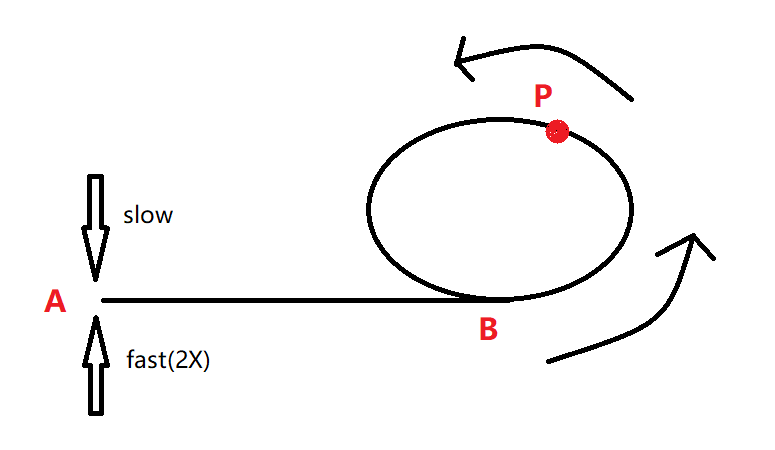
\includegraphics[width=0.7\textwidth]{Fast-and-slow-pointer.png}
	\caption{Fast-and-slow-pointer \label{fig:Fast-and-slow-pointer}}
\end{figure}

代码如下:
\lstinputlisting[language=C++, style=codestyle2]{code03/pollard-rho.cpp}

由于求$GCD$大概会有一个常数,考虑进一步优化。显然如果我们能求得$gcd(ab,N)>1$,那么也是找到了一个因子,只要$a,b$中某一个有$N$的因子即可。
所以我们可以先不急着做$GCD$,而是做一系列的$|t-s|$的连乘,到一定次数再做$GCD$。为了不溢出,我们使连乘的结果$mod\ N$,由欧几里得算法知答案不变。

\lstinputlisting[language=C++, style=codestyle2]{code03/pollard-rho-with-multi.cpp}

pollard-rho算法往往会和miller-rabin同时使用,比如章节题目\ref{prob:pollard}。
其要判断一个数是否是素数,若不是则输出其最大质因子。

代码如下,可作为模板,时间复杂度$O(T*\alpha*(N^{1\over 4}+log^2(N)))$。其中$T$表示数据组数,$\alpha$表示一个不小的常数。

\lstinputlisting[language=C++, style=codestyle2]{code03/luogu-p4718.cpp}

\section{离散对数}

现在我们来思考这样一个问题:

\begin{custom}{问题}
	给定$a,b,m$,求$a^x\equiv b \ (mod \ m)$的解$x$。
\end{custom}

\begin{solution}
	
	我们设$x=A\left \lceil \sqrt{m} \right \rceil -B$,其中$0\le B< \left \lceil \sqrt{m} \right \rceil$, $0< A\le \left \lceil \sqrt{m} \right \rceil+1$,这样化简后的方程是
	$$
	a^{A\left \lceil \sqrt{m} \right \rceil}\equiv b\cdot a^B \quad (mod \ m)
	$$
	由于$A$和$B$值域都是$O(\sqrt{m})$级别的,所以可以先计算右边部分的值,存入$Hash$表,然后从小到大枚举$A$计算左边的值,在$Hash$表中查找。
	(当然,可以这样做的原因是一定存在$a$的逆元)即只要$gcd(a,m)=1$,上面的方法就是有效的。所以当$m$是质数时,用这种方法(Baby Step Giant Step, bsgs)即可。
	
	{\heiti 当$m$不是质数时},我们要求解的是$a^x+km=b$,设$g=gcd(a,m)$,如果$g$不整除$b$,则无解,否则方程两边同除以$g$,得到$\frac{a}{g}a^{x-1}+k\frac{m}{g}=\frac{b}{g}$。
	这样便消去了m的一个因子,得到方程
	$$
	\frac{a}{g}a^{x-1}\equiv \frac{b}{g}\quad (mod \   \frac{m}{g})
	$$
	令${m}'=\frac{m}{g} ,\ b'=\frac{b}{g}(\frac{a}{g})^{-1}$, 得到
	$$
	a^{x'}\equiv b' \quad (mod \ m')
	$$
	于是可以递归,得到的解加1即$x=x'+1$为原方程的解。
	
	{\heiti 但是,进行一次这样的操作,新的方程不一定可以用bsgs求解,所以会进行多次。}
	
	如果中途出现$b'=1$则$x'=0$。
\end{solution}

时间复杂度  $O(\sqrt{m}log\sqrt{m})$,手写二分比unordered\_map会快一点。

\lstinputlisting[language=C++, style=codestyle2]{code03/bsgs.cpp}

注意到代码中有一个技巧,不用把每一步的逆元实际求出来,放到式子左边乘起来就行。
查表时,把初值设置为这个数$*a^{\left \lceil \sqrt{m} \right \rceil}$即可。


\section{原根}
\subsection{幂模$p$与原根}

如果$a$和$p$互素,费马小定理告诉我们,$a^{p-1} \equiv 1\ (mod\ p)$,那么这个指数$p-1$是唯一的使得结果为1的吗?
我们选择一些$a$和$p$来看一下,对于$a=3,p=7$,指数只有为6时才取到1,如表\ref{tab:root}。


\begin{table}[!htbp]
	\centering
	\caption{$a=3,\ p=7$ \label{tab:root}}
	\begin{tabular}{ccc}
		\midrule
		 $3^1\equiv 3(mod\ 7)$  & $3^2\equiv 2(mod\ 7)$ & $3^3\equiv 6(mod\ 7)$ \\
		 $3^4\equiv 4(mod\ 7)$    & $3^5\equiv 5(mod\ 7)$ & $3^6\equiv 1(mod\ 7)$ \\
		 \bottomrule
	\end{tabular}%
\end{table}%

再列多一点,如表\ref{tab:root2},从表中可以看出,似乎有这样的性质:
\begin{itemize}
	\item 对于任何底数,最小指数$e$整除$p-1$;
	\item 总有一些底数,指数需要到$p-1$。
\end{itemize}

\begin{table}[!htbp]
	\centering
	\caption{不同底数对应的最小指数 \label{tab:root2}}
	\begin{tabular}{ccc}
		\toprule
		$p=5$  & $p=7$ & $p=11$ \\
		\midrule
		$1^1\equiv 1(mod\ 5)$  & $1^1\equiv 1(mod\ 7)$ & $1^1\equiv 1(mod\ 11)$ \\
		$2^4\equiv 1(mod\ 5)$    & $2^3\equiv 1(mod\ 7)$ & $2^{10}\equiv 1(mod\ 11)$ \\
		$3^4\equiv 1(mod\ 5)$  & $3^6\equiv 1(mod\ 7)$ & $3^5\equiv 1(mod\ 11)$ \\
		$4^2\equiv 1(mod\ 5)$    & $4^3\equiv 1(mod\ 7)$ & $4^5\equiv 1(mod\ 11)$ \\
	                             & $5^6\equiv 1(mod\ 7)$ & $5^5\equiv 1(mod\ 11)$ \\
		    					& $6^2\equiv 1(mod\ 7)$ & $6^{10}\equiv 1(mod\ 11)$ \\
		  											& & $7^{10}\equiv 1(mod\ 11)$ \\
		   			  								& & $8^{10}\equiv 1(mod\ 11)$ \\
		   			  								& & $9^{5}\equiv 1(mod\ 11)$ \\
		   			  								& & $10^{2}\equiv 1(mod\ 11)$ \\
		\bottomrule
	\end{tabular}%
\end{table}%


为了方便,我们定义$a$模$p$的阶指$e_p(a)=[min\ e\ s.t.\ a^e\equiv 1(mod \ p)]$,其中$a$和$p$互质。另外,规定$e_p(a)\ge 1$,显然$e_p(a)\le p-1$。

\begin{theorem}{次数整除性质}{label}
	设a是不被素数$p$整除的整数,假设$a^n \equiv 1 \ (mod \ p)$,则次数$e_p(a)$整除$n$,特别地$e_p(a)$总整除$p-1$。
\end{theorem}

\begin{proof}
	次数$e_p(a)$的定义告诉我们
	$$
	a^{e_p(a)}\equiv 1 \ (mod \ p)
	$$
	假设$a^n\equiv 1(\ mod \ p)$,
	设$G=gcd(e_p(a),n)$,
	并设$(u,v)$是方程$e_p(a)u-nv=G$的正整数解(可知一定有解)。现在有两种不同的方法计算$a^{e_p(a)u}$:
	\begin{align*}
		a^{e_p(a)u}=(a^{e_p(a)})^u\equiv 1 \ (mod \ p)  \\
		a^{e_p(a)u}=a^{nv+G}\equiv a^G \ (mod \ p)  \\
	\end{align*}

	这表明$a^G\equiv 1 (\ mod \ p)$ ,所以必有$e_p(a)\le G$。
	
	另一方面$G \ | \ e_p(a)$,所以$G=e_p(a)\ ,\ e_p(a)\ | \ n$,证毕。
\end{proof}

{\heiti 现在我们的一个猜想得到了证明,来看另外一个:$e_p(a)=p-1$的底数$a$有什么规律。}

如果a是这样的数,则幂
$$
a^1,\ a^2,\ a^3,\ ...\ ,\ a^{p-2},\ a^{p-1}\quad (\ mod \ p)
$$
{\heiti 必须都是模$p$不同的。}[如果幂不是全不相同,则对某指数$1\le i <j\le p-1$有$a^i\equiv a^j \ (mod \ p)$,由于a,p互质,则有$1\equiv a^{j-i} \ (mod \ p)$,由于$j-i<p-1$,则矛盾]。

{\heiti 这$p-1$个不同的数取遍了$[1,p-1]$。}

{\heiti 这样的数很重要,为了方便,我们称这样的数$g$为模数$p$的原根,即$e_p(g)=p-1$。}

回顾前面的那张表\ref{tab:root2},5的原根是2,3\quad ;\quad 7的原根是3,5\quad ;\quad 11的原根是2,6,7,8。
可见原根可以不止一个,那到底有多少个?所有素数都有原根吗?

\begin{theorem}{原根定理}{label}
每个素数$p$都有原根。更精确地,有恰好$\varphi(p-1)$个原根。
\end{theorem}

神奇!尽管原根定理没有指出求$p$的原根的具体方法,但一旦能求得一个原根,就可以容易得求出其他原根(后面介绍)。求原根的常用方法是从小到大枚举正整数a=2,3,5,6......。{\heiti 因为原根的分布比较广}。(思考为什么没有4)。
为啥没4?因为$4^{\frac{(p-1)}{2}}\equiv 2^{p-1}\equiv 1 \ (mod \ p)$,即4一定不是原根。(可见2的高次幂都不是)

\begin{proof}
	原根定理的证明。
	
	对$1\sim p-1$之间的每个数$a$,$e_p(a) \ | \ (p-1)$ ,所以,对整数$p-1$的每个因子$d$,我们可能会问,有多少个$e_p(a)$等于$d$,由于要用,我们记这个数为$\psi (d),\ 1\le a <p$。 
	$\psi(p-1)$即为模数$p$的原根个数。
	
	设$n$是整除$p-1$的任何数,比如说$p-1=nk$,则可将多项式$X^{p-1}-1$分解成$X^{nk}-1=(X^n)^k-1=(X^n-1)((X^n)^{k-1}+(X^n)^{k-2}+...+(X^n)^2+X^n+1)$
	
	我们数一下这些多项式模$p$有多少个根。
	
	首先,$X^{p-1}-1\equiv 0 \ (mod \ p)$恰好有$p-1$个解,即$[1,p-1]$这些。
	
	另一方面,$(X^n-1)\equiv 0 \ (mod \ p)$至多有$n$个解,且
	$$
	(X^n)^{k-1}+(X^n)^{k-2}+...+(X^n)^2+X^n+1 \equiv 0 \ (mod \ p)
	$$
	至多有$nk-n$个解。
	
	因此我们得到:
	\begin{figure}[htbp]
		\centering
		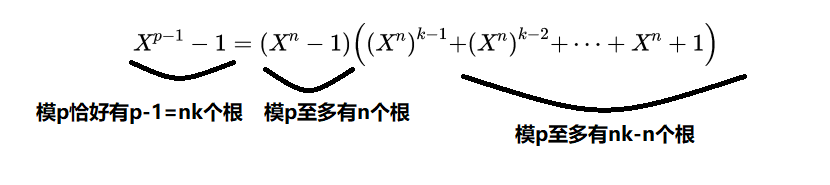
\includegraphics[width=0.7\textwidth]{prime-root.png}
		\caption{根的情况 \label{fig:prime-root}}
	\end{figure}

	上式要成立,$X^n-1$模$p$恰有$n$个根。这就证明了下述重要事实:
	
	{\heiti 如果$n \ | \ p-1$,则同余式$X^n-1\equiv 0 \ (mod \ p)$恰好有$n$个根满足$0\le X<p$。}
	
	现在再用另一种计数方法计数这个同余式的解的个数。如果$X=a$是一个解,则$a^n\equiv 1\ (mod \ p)$,因此$e_p(a)\ | \ n$,即$e_p(a)$对应$n$的一个因子$d$。
	从这个角度,$X^n-1\equiv 0 \ (mod \ p)$解($0\le X<p$)的个数等于:
	$$
		\sum_{d|n}\psi(d)=\psi(d_1)+\psi(d_2)+...+\psi(d_r)
	$$
	
	综合上面两个角度,我们得到一个结论:
	\begin{center}
	{\heiti 若$n$整除$p-1$,则$\sum_{d|n}\psi(d)=n$}
	\end{center}

	
	这个公式和欧拉函数的形式一样!首先,$\varphi(1)=1$,而$\psi(1)=1$,下面证明当$n=q$为素数时,$\psi(n)=\varphi(n)$。
	q的因数是1和q,所以$\psi(q)+\psi(1)=q=\varphi(q)+\varphi(1)$,由于$\psi(1)=\varphi(1)$,则$\psi(q)=\varphi(q)$。$n=q^2$和$n=q_1q_2$也可以类似证明。
	更正式地,可以给出归纳证明,这里不展示了。
	
	证毕。
\end{proof}

{\heiti 综上,我们已证明对整除$p-1$的每个整数$n$,恰好有$\varphi(n)$个底数$a$使得$e_p(a)=n$,取$n=p-1$,则$\varphi(p-1)$为原根个数。显然,每个素数至少有一个原根。}

\vbox{}

{\heiti 求原根,时间复杂度: 对于单个$p$,$O(\sqrt{p} + T*logn*logn)$   ;对于区间问题,可以做到$O(nlogn + \frac{n}{logn}*T*logn*logn)$,其中$T$表示平均意义下每个素数最小原根。
除以$logn$是因为素数的分布。}
\lstinputlisting[language=C++, style=codestyle2]{code03/primitive-root.cpp}

\subsection{原根与指标}
我们大概知道原根是啥了,那指标是什么呢?对于模数13,2是它的原根,那么$2^x\ mod \ 13$会取遍$[1,12]$里所有的数,$x\in [1,12]$。
{\heiti 而指标函数$I$就是从余数到指数的双射函数。}比如$2^4\equiv 3\ (mod\ 13)$,则$I(3) = 4$。



\begin{theorem}{指标法则}{label}
	指标满足下述法则:
		\begin{itemize}
			\item $I(ab)\equiv I(a)+I(b) \quad (mod \ p-1)$ \quad  乘积法则
			\item $I(a^k)\equiv k*I(a)  \quad (mod \ p-1)$ \quad  幂法则
		\end{itemize}
\end{theorem}

\begin{note}
	模数是$p-1$。
\end{note}

\begin{proof}
	 $g^{I(ab)}\equiv ab\equiv g^{I(a)}g^{I(b)}\equiv g^{I(a)+I(b)}\quad (mod \ p)$
	
	这意味着$g^{I(ab)-I(a)-I(b)}\equiv 1\ (mod \ p)$,又$g$是原根,则$I(ab)-I(a)-I(b)$是$p-1$的倍数。
	
	所以乘积法则得证。幂法则同理。
\end{proof}

\vbox{}

利用指标这个工具,可以方便地解一些高次同余方程。

\begin{custom}{问题}
求同余式$3x^{30}\equiv 4\ (mod \ 37)$。
\end{custom}

\begin{solution}
	使用乘积法则和幂法则:
$$
\begin{aligned} I\left(3 x^{30}\right) &=I(4) \\ I(3)+30 I(x) & \equiv I(4)(\bmod 36) \\ 26+30 I(x) &\equiv2(\bmod 36) \\ 30 I(x) & \equiv-24\equiv12(\bmod 36) \end{aligned}
$$
对于最后一个式子,是一个同余方程,由于$gcd(30,36)=6\ |\ 12$,则其有解,且有6个不同余解。
我们求得
$$
I(x)\equiv 4,\ 10,\ 16,\ 22,\ 28,\ 34 \quad (mod \ 36)
$$
再查双射表得到对应的值,有6个解$16,\ 25,\ 9,\ 21,\ 12,\ 28$。
\end{solution}

可以看到指标法的优点在于将{\heiti 幂运算转为乘法,将乘法转为加法}。这一点和对数函数很像:
$$
\begin{aligned} \log (a b) &=\log (a)+\log (b) \\ \log \left(a^{k}\right) &=k \log (a) \end{aligned}
$$

类似这一题的同余式称为剩余问题,下一章我们就来研究一下。这一章就到这。


\vbox{}

\vbox{}

\begin{problemset}
	\item \href{http://poj.org/problem?id=2891}{Strange Way to Express Integers \quad POJ2891 \quad 同余方程组,模数不一定互质}  
	\item \href{https://cn.vjudge.net/problem/Gym-101550E#}{Exponial \quad 欧拉降幂}
	\item \href{http://acm.hdu.edu.cn/showproblem.php?pid=4910}{Problem about GCD \quad 威尔逊定理的应用}
	\item \href{https://vjudge.net/problem/HDU-5391}{Zball in Tina Town \quad 威尔逊定理 \quad 素性测试}
	\item \href{https://www.luogu.org/problem/P4718}{【模板】Pollard-Rho算法 \quad 素性测试 \quad Pollard\_Rho质因数分解 \label{prob:pollard}}
	\item \href{https://www.spoj.com/problems/MOD/}{MOD - Power Modulo Inverted \quad 离散对数}
	\item 对任何正整数$k$,求$1^k+2^k+3^k+...+(p-1)^k\ (mod\ p)$的值。 \  ans:0 \href{https://math.stackexchange.com/questions/1049420/for-any-positive-number-k-find-the-value-of-1k-2k-3k-p-1kmod?r=SearchResults#}{solution}
	\item (2017四川省赛K.2017)给你$n$(不超过200w)个数,和一个数$r$,问你有多少种方案,使得你取出某个子集,能够让它们的乘积$mod \ 2017$等于$r$。由于
	方案数众多,最后只需要输出答案的奇偶性即可。\href{https://www.cnblogs.com/autsky-jadek/p/7496328.html}{\quad 原根}
\end{problemset}


\chapter{剩余}

\begin{introduction}
\item 二次互反律
\item 勒让德符号
\item 二次剩余
\item N次剩余
\end{introduction}

\vbox{}

第三章中我们已经知道了如何解线性同余式,现在让我们来考虑更高次的同余方程,首先来看下二次同余方程。

\section{二次剩余}
在发现规律前,人们总要先做一些实验。取模数为7,取遍底数:
$$
\begin{aligned} 0^{2} & \equiv 0(\bmod 7) \\ 1^{2} & \equiv 1(\bmod 7) \\ 2^{2} & \equiv 4(\bmod 7) \\ 3^{2} & \equiv 2(\bmod 7) \\ 4^{2} & \equiv 2(\bmod 7) \\ 5^{2} & \equiv 4(\bmod 7) \\ 6^{2} & \equiv 1(\bmod 7) \end{aligned}
$$

我们可以看到余数并不会包含所有底数,而且不包含的还挺多。

再取多一点模数,如图\ref{fig:quadratic-residue-example}。

\begin{figure}[htbp]
	\centering
	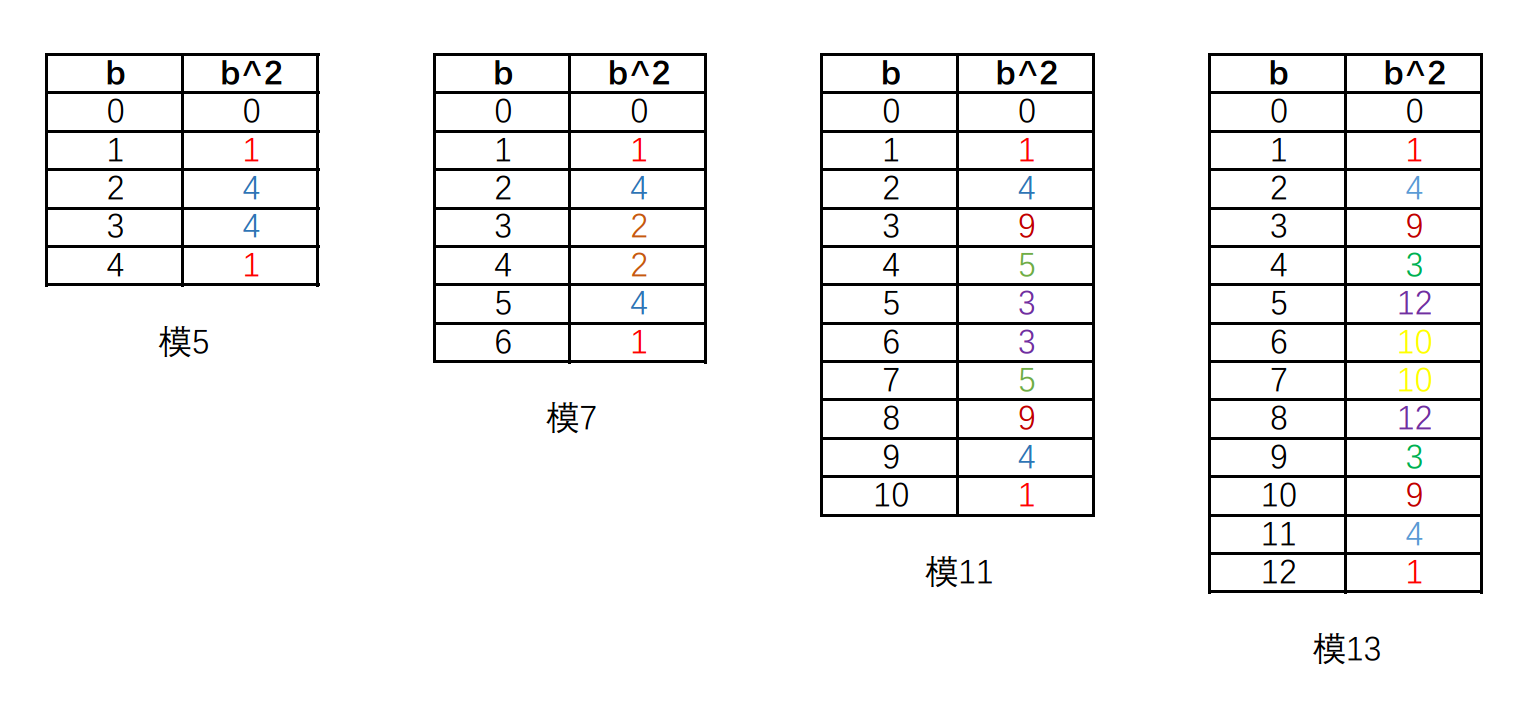
\includegraphics[width=1.0\textwidth]{quadratic-residue-example.png}
	\caption{二次剩余的模式 \label{fig:quadratic-residue-example}}
\end{figure}

可以看到上下的对称性,即数$b$的平方剩余与数$p-b$的平方剩余是模$p$相同的。这一点也比较好证明:
$$
p^2+b^2-2pb=(p-b)^2\equiv b^2 \quad (mod \ p)
$$

因此,若要列出模$p$的所有(非零)平方剩余,只需要计算出其中的一半:

$$
1^2\ (mod \ p)\ ,\ 2^2\ (mod \ p)\ ,\ ...\ ,\ (\frac{p-1}{2})^2 \ (mod \ p)
$$

那如何快速判断一个数是否是二次剩余呢?在探索之前,我们先明确一下定义:

\begin{definition}{二次剩余与二次非剩余}{label}
\begin{itemize}
\item 与一个平方数模$p$同余的非零数称为模$p$的二次剩余
\item 不与任何一个平方数模$p$同余的数称为模$p$的二次非剩余
\item 将二次剩余简记为$QR$,二次非剩余简记为$NR$
\item 与0模$p$同余的数既不是$QR$,也不是$NR$
\end{itemize}
\end{definition}


\begin{theorem}{二次剩余性质}{label}
设$p$为一个奇素数,则恰有$\frac{p-1}{2}$个模$p$的二次剩余,且恰有$\frac{p-1}{2}$个模$p$的二次非剩余。
\end{theorem}

\begin{proof}
由前面的结论知道,只要证明$1^2,2^2,...,(\frac{p-1}{2})^2  \ mod \ p$是两两不同的。

假设$b_1,b_2$是$[1,\frac{p-1}{2}]$之间的数,且满足$b_1^2\equiv b_2^2\ (mod \ p)$。

我们要证明$b_1=b_2$。

由于$b_1^2\equiv b_2^2\ (mod \ p)$,得到$p\ | \ (b_1^2-b_2^2)=(b_1-b_2)(b_1+b_2)$,

然而$b1+b2$显然不能被$p$整除,所以$b_1-b_2=0$,证毕。
\end{proof}

\vbox{}

QR与NR有什么关系呢?一个不难想到的结论是$QR*QR=QR$。(等于号表示仍为$QR$)
因为平方数乘平方数仍为平方数,所以两个二次剩余乘积模$p$仍为二次剩余。那么其他的组合呢?
经过一些小的表观察,可以得到:

$$
QR*QR=QR  ,\quad QR*NR=NR  ,\quad NR*NR=QR
$$

在验证后面两个关系之前,我们先来看下原根与二次剩余的关系,原根是分析一些问题时好用的工具,
也许能帮助我们证明。

设$g$是模$p$的一个原根,那么$g$的幂:
\begin{align}
g\ ,\ g^2\ ,\ g^3\ ,\ ...\ ,\ g^{p-1} \label{formula:primeroot-residue}
\end{align}

可以给出$p$的所有非零剩余,即$[1,p-1]$。其中一半是二次剩余,一半是二次非剩余。
如何确定哪些是$QR$,哪些是$NR$呢?

显然$g$的每个偶次幂一定是一个$QR$,即$g^{2k}$。

注意到在式子\ref{formula:primeroot-residue}中恰有一半是偶次幂,所以{\heiti $g$的偶次幂给出了所有的二次剩余}。而剩下的奇次幂必定是二次非剩余。

同时,也可以用指标来描述,二次剩余是指标$I(a)$为偶数的那些数$a$;二次非剩余是指标$I(a)$为奇数的那些数$a$。
利用二次剩余与二次非剩余的这种指标性质,可以很简单地证明二次剩余的乘法法则。

\begin{theorem}{二次剩余乘法法则--表达方式1}{residue1}
设$p$为素数,则
\begin{itemize}
\item 两个模$p$的二次剩余的积是二次剩余
\item 二次剩余与二次非剩余的积是二次非剩余
\item 两个二次非剩余的积是二次剩余
\end{itemize}
即
$$
QR*QR=QR  ,\quad QR*NR=NR  ,\quad NR*NR=QR
$$
\end{theorem}

\begin{proof}
对与$p\ (p>2)$互素的任意两个数$a,b$,由指标的乘积法则知$I(ab)\equiv I(a)+I(b) \quad (mod \ p-1)$,
从而有$I(ab)\equiv I(a)+I(b) \quad (mod \ 2)$。 后面的证明就很自然了。可以讨论定理\ref{thm:residue1}中的三种情况。
\end{proof}

\vbox{}

对于定理\ref{thm:residue1},你肯定会想到$QR,NR$和$+1,-1$的性质类似。
许多年前,勒让德(Adrien-Marie Legendre)也想到了,而且还引入了一种符号:


\begin{definition}{勒让德符号}{label}
$a$模$p$的勒让德符号是
\begin{align*}
\left(\frac{a}{p}\right)=\left\{\begin{matrix}
1 & \quad  if\ a\ is\ Quadratic\ residue \\  
-1& \quad  else
\end{matrix}\right.
\end{align*}
\end{definition}

利用勒让德符号,二次剩余的乘法法则可用一个公式表示。

\begin{theorem}{二次剩余乘法法则--表达方式2}{residue2}
设$p$为素数,则
$$
\left(\frac{a}{p}\right)\left(\frac{b}{p}\right)=\left(\frac{ab}{p}\right)
$$
\end{theorem}

勒让德符号使计算可以更直观,比如
$$
\left(\frac{75}{97}\right)=\left(\frac{3\cdot5\cdot5}{97}\right)=\left(\frac{3}{97}\right)\left(\frac{5}{97}\right)\left(\frac{5}{97}\right)
$$
而
$$
\left(\frac{5}{97}\right)\left(\frac{5}{97}\right)=1
$$
所以
$$
\left(\frac{75}{97}\right)=\left(\frac{3}{97}\right)=1 \quad   (3\ is\ QR)
$$

这里能够判断出3是模97的一个$QR$有些幸运($10^2$),我们似乎还没有回答如何快速计算一个数是否是二次剩余,即如何快速计算勒让德符号。

\section{二次互反律}
通过前一节的讨论,我们清楚了对于任何一个奇素数,$[1,p-1]$有一半是二次剩余。
现在先换个角度,考虑对于一个数$a$,看看对于哪些$p$,这个数是$QR$。

我们先令$a=-1$,看对于哪些素数$p$,同余式$x^2\equiv -1\ (mod \ p)$有解。
或者说,对哪些素数,$\left( \frac{-1}{p} \right)=1$。同样,通过列出小的数据,可以看出,
{\heiti 若$p$与1模4同余,则$-1$似乎是$p$的$QR$;若$p$与3模4同余,则$-1$似乎是$NR$。}

用来证明这个猜想的工具称为“费马小定理的平方根”,即考虑$A=a^\frac{p-1}{2} \ mod \ p$值为多少?

\begin{theorem}{欧拉准则}{label}
设$p$为素数,则
$$
a^\frac{p-1}{2}\equiv  \left( \frac{a}{p} \right) \quad mod \ p
$$
\end{theorem}

\begin{proof}
令$A=a^\frac{p-1}{2}$,显然$A^2\equiv 1 \ mod \ p$,因此$p$整除$(A-1)(A+1)$。
从而$p$要么整除$(A-1)$要么整除$(A+1)$,因此$A$要么和$1$模$p$同余,要么和$-1$。


当$a$是$QR$时,则$a\equiv g^{2k}\ (mod \ p)$ ,则$a^{\frac{p-1}{2}}\equiv (g^{p-1})^k\equiv 1\ (mod \ p)$;
当$a$是$NR$时,则$a\equiv g^{2k+1} \ (mod \ p)$,则$a^{\frac{p-1}{2}}\equiv g^{\frac{p-1}{2}} \ (mod \ p)$。
由前面讨论知道,$a^{\frac{p-1}{2}}$要么和$1$模$p$同余,要么和$-1$。这里由于$g$是原根,则和$1$模$p$同余的最小次幂只能是$p-1$。
所以这里$a^{\frac{p-1}{2}}\equiv -1 \ (mod \ p)$。
证毕。
\end{proof}


有了欧拉准则,就可以轻松的判断$-1$是不是$p$的二次剩余了:

\begin{theorem}{二次互反律---part one}{label}

设$p$为素数,{\heiti 若$p$与1模4同余,则$-1$是$p$的$QR$;若$p$与3模4同余,则$-1$是$NR$。}

用勒让德符号表示如下:
$$
\left(  \frac{-1}{p}  \right)= \left\{\begin{matrix}
1   \quad if\ p\equiv 1 \ (mod \ 4) \\ 
-1 \quad if\ p\equiv 3 \ (mod \ 4)
\end{matrix}\right.
$$
\end{theorem}

\begin{proof}
带入欧拉准则即证。
\end{proof}

\vbox{}

下面考虑$a=2$的情况。如果直接使用欧拉准则,即$2^{\frac{p-1}{2}} \ mod \ p$,似乎不能看出结果是1还是-1。
高斯提出了一个方法,可以简单地知道$2^{\frac{p-1}{2}} \ mod \ p$的值是-1还是1,其结论和二次互反律part one一样简单:


\begin{theorem}{二次互反律---part two}{label}
$$
\left(  \frac{2}{p}  \right)= \left\{\begin{matrix}
1   \quad if\ p\equiv 1\ or\ 7 \ (mod \ 8) \\ 
-1 \quad if\ p\equiv 3\ or\ 5\ (mod \ 8)
\end{matrix}\right.
$$
\end{theorem}

\begin{proof}
利用欧拉准则知,需要寻找$2^{\frac{p-1}{2}} \ mod \ p$结果的模式。
$p$是一个素数,令$P=\frac{p-1}{2}$,从偶数$2,4,6,...,p-1$开始,将它们相乘,并从每个数中提出2因子,可得
$$
2*4*6*\cdots*(p-1)=2^P*P!
$$
然后再对$2,4,6,...,p-1$进行模$p$化简,使其全部落在$[-P,P]$之间,乘起来。比较这两个乘积,可得
$$
2^P*P!\equiv (-1)^{Number\ of\ negative\ signs}* P! \quad (mod \ p)
$$
负号的个数是指对$2,4,6,...,p-1$进行模$p$化简后落在$[-P,-1]$之间的个数。消去$P!$,得
$$
2^{\frac{p-1}{2}}\equiv  (-1)^{Number\ of\ negative\ signs}  \quad  (mod \ p)
$$
于是当负数的个数为偶数时,$2$是$p$的二次剩余。而这里负数的个数和$p\ mod\ 8$相关,具体如定理中所示。
\end{proof}

\vbox{}

现在总结一下。对于一个给定的数$a$,我们要确定哪些素数$p$以$a$为二次剩余。上面解决了$a=-1$和$a=2$时的问题。
这个时候我们可以通过查看$p\%m$的一些结果得出$a$是否是$QR$或$NR$,且$m$较小,为$4$和$8$。
下面要解决的是其他$a$值的勒让德符号$(\frac{a}{p})$的计算问题。({\heiti 当然,你可以直接使用欧拉准则
去计算},但下面的方法还是很值得知晓)

例如,假设要计算$(\frac{70}{p})$,由前面的二次剩余乘法法则知,$(\frac{70}{p})=(\frac{2}{p})(\frac{5}{p})(\frac{7}{p})$,
怎么计算$(\frac{5}{p})$和$(\frac{7}{p})$呢?

概括来说,怎么计算$(\frac{q}{p})$呢?其中$q$也为素数。因为由乘法法则知,素数可以解决后,整数都可以解决。

通过打表观察后(此处略去500字......),可以得到对于一些$p,q$,有$\left( \frac{q}{p} \right)=\left( \frac{p}{q} \right)$;但有些不是,但不是的竟然都是$\left( \frac{q}{p} \right)=-\left( \frac{p}{q} \right)$。
这其中有没有模式呢?有的。

\begin{theorem}{二次互反律}{label}
$$
\left(  \frac{-1}{p}  \right)= \left\{\begin{matrix}
1   \quad if\ p\equiv 1 \ (mod \ 4) \\ 
-1 \quad if\ p\equiv 3 \ (mod \ 4)
\end{matrix}\right.
$$
$$
\left(  \frac{2}{p}  \right)= \left\{\begin{matrix}
1   \quad if\ p\equiv 1\ or\ 7 \ (mod \ 8) \\ 
-1 \quad if\ p\equiv 3\ or\ 5\ (mod \ 8)
\end{matrix}\right.
$$
$$
\left(\frac{q}{p}\right)=\left\{\begin{array}{c}{\left(\frac{p}{q}\right)}\quad if\ p\equiv1\ (mod\ 4)\ or\ q\equiv1\ (mod\ 4) \\ {-\left(\frac{p}{q}\right) \quad if\ p\equiv3\ (mod\ 4)\ and\ q\equiv3\ (mod\ 4) }\end{array}\right.
$$
\end{theorem}

\begin{proof}
前两部分已经证明,最后一个部分感兴趣的读者可以自行查阅资料。
\end{proof}

\vbox{}

二次互反律不仅很美,也很实用。
它使我们可以翻转勒让德符号$\left(\frac{q}{p}\right)$,用$\pm \left(\frac{p}{q}\right)$来替代它,然后可以模$q$化简$p$,并不断重复此过程,这样会使$p,q$急剧下降。

所以,计算勒让德符号的困难之处不是二次互反律的使用,而是对数字的因式分解。

如果不分解,继续做下去,这样答案是否正确呢?

{\heiti 正确!} 也就是说对于$\left(\frac{q}{p}\right)$,之前是$p,q$为素数,现在是对任意的正奇数$a$和$b$,可以给勒让德符号$\left(\frac{a}{b}\right)$指定一个值,反复使用广义二次互反定律来计算结果。这种广义勒让德符号常称作{\heiti 雅克比符号}。

\begin{theorem}{广义二次互反律}{label}
设$a,b$为正奇数,则
$$
\left(  \frac{-1}{b}  \right)= \left\{\begin{matrix}
1   \quad if\ b\equiv 1 \ (mod \ 4) \\ 
-1 \quad if\ b\equiv 3 \ (mod \ 4)
\end{matrix}\right.
$$
$$
\left(  \frac{2}{b}  \right)= \left\{\begin{matrix}
1   \quad if\ b\equiv 1\ or\ 7 \ (mod \ 8) \\ 
-1 \quad if\ b\equiv 3\ or\ 5\ (mod \ 8)
\end{matrix}\right.
$$
$$
\left(\frac{a}{b}\right)=\left\{\begin{array}{c}{\left(\frac{b}{a}\right)}\quad if\ a\equiv1\ (mod\ 4)\ or\ b\equiv1\ (mod\ 4) \\ {-\left(\frac{b}{a}\right) \quad if\ a\equiv3\ (mod\ 4)\ and\ b\equiv3\ (mod\ 4) }\end{array}\right.
$$
\end{theorem}

\begin{note}
只允许当$a$是正奇数的时候翻转$a,b$,这一点极为重要。当$a$是偶数时,可以分解出因子2;当$a$是负数时,可以分解出因子$-1$。
\end{note}

\vbox{}

使用二次互反律求解勒让德符号,时间复杂度  $O(logb)$。

{\heiti 当然也可以直接用欧拉准则,快速幂即可。}

\lstinputlisting[language=C++, style=codestyle2]{code04/Legendre.cpp}

现在我们可以快速计算勒让德符号了(两种方法)。{\heiti 但知道有解还是不够的,往往我们想知道解是什么。}


\section{求解二次剩余}
Cipolla's algorithm是求解二次剩余的经典方法。
\begin{theorem}{Cipolla's algorithm}{Cipolla}
现有同余式$x^2\equiv n\ (mod\ p)$,其中$x,n\in \mathcal{F}_p$,$p$是奇素数,$\mathcal{F}_p$是有$p$个元素的有限域:$\{0,1,...,p-1\}$。
\begin{enumerate}
\item 寻找一个$a\in \mathcal{F}_p$,使得$a^2-n$是非二次剩余。(随机寻找即可,期望随机次数为2)
\item 在域$\mathcal{F}_{p^2}=\mathcal{F}_p(\sqrt{a^2-n})$中计算$x = (a+\sqrt{a^2-n})^{(p+1)/2}$即为满足$x^2=n$的一个解。
\end{enumerate}
\end{theorem}

在证明前,我们先来看一个例子。注意第二步骤之前所有元素都是在域$\mathcal{F}_{13}$中,第二步中在域$\mathcal{F}_{13^2}$中。

寻找$x^2=10$的所有解。

在执行算法前,你可以先用欧拉准则或者二次互反律计算一下$\left(  \frac{10}{13}  \right)$是否为1,若不是1,则无解;若是1,执行下面算法。

\begin{enumerate}
\item 随机寻找一个$a\in \mathcal{F}_{13}$,使得$a^2-10$是非二次剩余。假如随机到$a=2$,则$a^2-10$为$7$,$\left(  \frac{7}{13}  \right)=-1$,
满足要求。
\item 计算$x = (a+\sqrt{a^2-n})^{(p+1)/2} = (2+\sqrt{-6})^7$。
$$
\begin{array}{l}{(2+\sqrt{-6})^{2}=4+4 \sqrt{-6}-6=-2+4 \sqrt{-6}} \\ {(2+\sqrt{-6})^{4}=(-2+4 \sqrt{-6})^{2}=-1-3 \sqrt{-6}} \\ {(2+\sqrt{-6})^{6}=(-2+4 \sqrt{-6})(-1-3 \sqrt{-6})=9+2 \sqrt{-6}} \\ {(2+\sqrt{-6})^{7}=(9+2 \sqrt{-6})(2+\sqrt{-6})=6}\end{array}
$$
所以$x=6$是一个解,当然$(-6)\ mod\ 13 = 7$也是一个解。
\end{enumerate}

\vbox{}

\begin{proof}
Cipolla's algorithm正确性的证明。

{\heiti Part I\quad 证明$\mathcal{F}_{p^2}=\mathcal{F}_p(\sqrt{a^2-n})=\{x+y\sqrt{a^2-n}:x,y\in \mathcal{F}_p\}$确实是一个域。}

为了记号方便,令$\omega = \sqrt{a^2-n}$,由于$a^2-n$是非二次剩余,所以在$\mathcal{F}_{p}$中是没有平方根的。这里$\omega$可以类比复数域中的$i$。

$\mathcal{F}_{p^2}$中的加法被定义为:
$$
\left(x_{1}+y_{1} \omega\right)+\left(x_{2}+y_{2} \omega\right)=\left(x_{1}+x_{2}\right)+\left(y_{1}+y_{2}\right) \omega
$$

乘法被定义为:
$$
\left(x_{1}+y_{1} \omega\right)\left(x_{2}+y_{2} \omega\right)=x_{1} x_{2}+x_{1} y_{2} \omega+y_{1} x_{2} \omega+y_{1} y_{2} \omega^{2}=\left(x_{1} x_{2}+y_{1} y_{2}\left(a^{2}-n\right)\right)+\left(x_{1} y_{2}+y_{1} x_{2}\right) \omega
$$

可交换、可结合、可分配都比较显然。加法幺元是$0+0\omega$,乘法幺元是$1+0\omega$。
下面证明加法和乘法逆元的存在。显然$x+y\omega$的加法逆元是$-x-y\omega$。对于乘法,记$\alpha = x_1+y_1\omega,\ \alpha^{-1}=x_{2}+y_{2} \omega$,则有:
$$
\left(x_{1}+y_{1} \omega\right)\left(x_{2}+y_{2} \omega\right)=\left(x_{1} x_{2}+y_{1} y_{2}\left(a^{2}-n\right)\right)+\left(x_{1} y_{2}+y_{1} x_{2}\right) \omega=1
$$

通过对应系数可得两个方程:
$$
\left\{\begin{array}{l}{x_{1} x_{2}+y_{1} y_{2}\left(a^{2}-n\right)=1} \\ {x_{1} y_{2}+y_{1} x_{2}=0}\end{array}\right.
$$

解得:
$$
\begin{array}{l}{x_{2}=-y_{1}^{-1} x_{1}\left(y_{1}\left(a^{2}-n\right)-x_{1}^{2} y_{1}^{-1}\right)^{-1}} \\ {y_{2}=\left(y_{1}\left(a^{2}-n\right)-x_{1}^{2} y_{1}^{-1}\right)^{-1}}\end{array}
$$

也就是说$x_2,\ y_2$确实存在,因为其表达式中的元素均在$\mathcal{F}_{p}$中。

Part I证毕,$\mathcal{F}_{p^2}$确实是一个域。

\vbox{}

{\heiti Part II\quad 证明对于域中的每个元素,有$x+y \omega \in \mathcal{F}_{p^{2}}:(x+y \omega)^{p}=x-y \omega$。}

首先在模$p$意义下有$(a+b)^p = a^p + b^p$,$x^p=x$,$\omega^{p-1}=\left(\omega^{2}\right)^{\frac{p-1}{2}}=-1 \ $ ($\omega^2=a^2-n$是非二次剩余,欧拉准则)。
所以
$$
(x+y \omega)^{p}=x^{p}+y^{p} \omega^{p}=x-y \omega
$$

Part II证毕。

\vbox{}

{\heiti Part III\quad 证明若$x_{0}=(a+\omega)^{\frac{p+1}{2}} \in \mathcal{F}_{p^{2}}$,则有$x_{0}^{2}=n \in \mathcal{F}_{p}$。}

$$
x_{0}^{2}=(a+\omega)^{p+1}=(a+\omega)(a+\omega)^{p}=(a+\omega)(a-\omega)=a^{2}-\omega^{2}=a^{2}-\left(a^{2}-n\right)=n
$$

注意上面的计算都发生在域$\mathcal{F}_{p^{2}}$中,所以$x_0\in \mathcal{F}_{p^{2}}$。由拉格朗日定理,在任何域上,$n$阶多项式最多有$n$个根。在$\mathcal{F}_{p}$上,$x^2-n$有两个
根,这些根在$\mathcal{F}_{p^{2}}$上同样也是根。所以在$\mathcal{F}_{p^{2}}$上$x^2-n$的两个根$x_0,\ -x_0$也是$\mathcal{F}_{p}$上$x^2-n$的根。

Part III证毕。

更多资料可以查看\href{https://en.wikipedia.org/wiki/Cipolla\%27s_algorithm}{https://en.wikipedia.org/wiki/Cipolla\%27s\_algorithm}
\end{proof}

\vbox{}

{\heiti 时间复杂度:$O(logp)$,常数较大,因为域$\mathcal{F}_{p^{2}}$中运算取模较多。}

模数为素数。
\lstinputlisting[language=C++, style=codestyle2]{code04/quad-res.cpp}

\vbox{}

{\heiti 如果模数是质数幂呢?}

设$q=p^k$,考虑求解$x^2\equiv n\ (mod\ q)$。当$n\equiv 0\ (mod\ p^k)$时,解为$x \equiv 0\left(\bmod p^{\lceil k / 2\rceil}\right)$。
否则可令$n=p^{r} a,\ p \nmid a,\ 0 \leqslant r<k$,有解时需要$r$为偶数,令$x=p^{r/2}x'$,则$x'^2\equiv a\ (mod\ p^{k-r})$。

所以只要考虑$x^2\equiv a\ (mod\ q)$,且$p\nmid a$的情况即可。下面分$p=2$和$p>2$两种情况讨论。

\begin{enumerate}
\item {\heiti 模2的幂。}$x^{2} \equiv a(\bmod\ q), q=2^{k}, 2\nmid a$。$q=4$时,有解当且仅当$a\equiv 1\ (mod\ 4)$,解为$x\equiv 1,3\ (mod\ 4)$。

下面考虑$q\ge8$的情况。由于任意奇数的平方模$8$余1,于是需有$a\equiv 1\ (mod\ 8)$。此时,$x^2\equiv a\ (mod\ q)$恰有4个解$\pm x_{k}, \pm\left(q / 2-x_{k}\right)$。
\begin{proof}
$q=8$时,4个解分别为$x \equiv \pm 1, \pm 3(\bmod 8)$。下面进行归纳。设$x^{2} \equiv a\left(\bmod\ 2^{k}\right)$的4个解为$\pm x_{k}, \pm\left(2^{k-1}-x_{k}\right)$,则
$$
\begin{aligned} & x_{k}^{2}-\left(2^{k-1}-x_{k}\right)^{2} \\=&\left(2 x_{k}-2^{k-1}\right) 2^{k-1} \\ \equiv & x_{k} 2^{k} \quad\left(\bmod\ 2^{k+1}\right) \\ \equiv & 2^{k} \quad\left(\bmod\ 2^{k+1}\right) \end{aligned}
$$
于是$x_{k}, 2^{k-1}-x_{k}$中恰有一个可以作为$x_{k+1}$,使得$x_{k+1}^{2} \equiv a\left(\bmod\ 2^{k+1}\right)$。又由$\left(2^{k}-x_{k+1}\right)^{2} \equiv x_{k+1}^{2}\left(\bmod\ 2^{k+1}\right)$即得另外两个解。证毕。
\end{proof}

\item {\heiti 模奇素数的幂。}$x^{2} \equiv a(\bmod\ q), q=p^{k}, p \nmid a$。当且仅当$a$是$p$的二次剩余时,上式有解。有解时恰有两个解$\pm x_{k}$。
\begin{proof}
使用归纳法。若$x_{k}^{2} \equiv a\left(\bmod\ p^{k}\right)$,设
$$
\begin{aligned} x_{k+1} &=x_{k}+t p^{k}\left(\bmod\ p^{k+1}\right), t=0,1, \cdots, p-1 \\ x_{k+1}^{2} &=x_{k}^{2}+t^{2} p^{2 k}+2 x_{k} t p^{k} \\ & \equiv x_{k}^{2}+2 x_{k} t p^{k}\left(\bmod\ p^{k+1}\right) \\ & \equiv a\left(\bmod\ p^{k+1}\right) \end{aligned}
$$
于是
$$
2x_kt\equiv (a-x_k^2)/p^k\ (mod\ p)
$$
解出$t$即可得到对应的$x_{k+1}$。
证毕。
\end{proof}
\end{enumerate}

\vbox{}

{\heiti 如果模数是合数,将模数分解后分别计算,再用中国剩余定理合并。}

参考资料:\href{https://max.book118.com/html/2018/0525/168640677.shtm}{jcvb\quad 二次剩余相关}

\section{求解N次剩余}
\begin{custom}{问题}
	给定$N,a,p$,求出$x^N\equiv a\ (mod \ p)$在模$p$意义下的所有解(其中$p$是素数) 。
\end{custom}

\begin{solution}
	如果能找到原根$g$,则$\{1,2,..,.p-1\}$与$\{g^1,g^2,...,g^{p-1}\}$之间就建立了双射关系。
	
	令$g^y=x,\ g^t=a$,$x^N\equiv a\ (mod \ p)$ ,则有
	$$
	g^{y*N}\equiv g^t  \quad (mod \ p)
	$$
	因为$p$是素数,所以方程左右都不会为0。原问题转化为:
	$$
	N*y\equiv t\ (mod \ (p-1))
	$$
	由于$N,p$已知,则上式为解模线性方程。
	
	而$t$的值,由$g^t\equiv a \ (mod\ p)$,用解离散对数的方法求出。
\end{solution}

输入:$1 \le a,\ N < p \le 10^9$,$p$为素数。

{\heiti 时间复杂度}  $O(\sqrt{p}log(\sqrt{p}))$ 

\lstinputlisting[language=C++, style=codestyle2]{code04/N-res.cpp}

{\heiti 如果模数是非素数呢?}

模数非素数:时间和素数一样,甚至更低,因为分解质因数处理的时候规模较小,最后中国剩余定理合并。
\lstinputlisting[language=C++, style=codestyle2]{code04/N-res-notprime.cpp}

\begin{example}
	已知$x^{2^{30}+3}\ mod\ n = c$,给定$c,n$,其中$n$是两个相邻素数($p \in [10^5, 10^9]$)的乘积。求解$x$,题目保证在模意义下只有一个解。
	$10^5$组测试数据。
	(\href{https://codeforces.com/gym/102055/problem/K}{CCPC2018-Final Mr. Panda and Kakin})
\end{example}

\begin{solution}
	注意到这里$2^{30}+3$和$\phi(n)$一定互质,所以可以直接求$2^{30}+3$模$\phi(n)$下的逆元,最后两边做逆元次方即得答案。
	
	注意要使用$O(1)$快速乘,否则超时。
\end{solution}

\lstinputlisting[language=C++, style=codestyle2]{code04/Kakin.cpp}

\begin{problemset}
	\item \href{https://www.luogu.org/problem/P5491}{二次剩余 \quad 洛谷P5491 \quad 模板}
	\item x  
\end{problemset}
\chapter{积性函数}

\begin{introduction}
	\item xxx
\end{introduction}


\section{因子次幂和函数}


\section{欧拉函数}


\section{莫比乌斯函数}


\section{莫比乌斯反演}


\section{积性函数与狄利克雷卷积}


\section{积性函数前缀和}


\section{杜教筛}


\section{拓展埃氏筛}
拓展埃氏筛(Extended Eratosthenes Sieve)似乎最早由min25引入竞赛圈(因此也常被称为min25筛),可以在{\heiti 低于线性的时间}内求得积性函数(一些非积性函数也可以)的前缀和。
由于其方法简单且灵活性高,近年来经常在算法竞赛中出现,下面就来介绍一下EES。

首先要介绍的是在EES中要使用到的一个前置算法,叫做The Meissel, Lehmer, Lagarias, Miller, Odlyzko Method{\heiti (MLLMO Method)},论文\cite{Deleglise1996Computing}中
对其进行了系统介绍,有兴趣的可以继续阅读。

\subsection{MLLMO Method}
MLLMO Method要解决的是这样一个问题:
求解
$$
\sum_{i=2}^n[i\in Prime]F(i)
$$
其中$F(x) = x^k$,即求解
$$
\sum_{i=2}^n[i\in Prime]\ i^k
$$
设$P_j$表示第$j$个质数,$P_1=2,\ P_2=3\ ...$,特殊地$P_0$可以认为是$0$。

MLLMO Method用动态规划的思想解决这个问题:

设
$$
dp(n,j)=\sum_{i=2}^ni^k\ [\ i\in Prime\ or \ min(p)>P_j,\ where\ p|i\ and\ p\in Prime\ ]
$$
也就是说$i$是质数,或者合数$i$的最小质因子大于$P_j$时对$dp(n,j)$有贡献。

那$dp(n,0)$即为$\sum_{i=2}^n\ i^k$。下面考虑如何进行转移。

{\heiti 1.假设$P_j^2>n,\ P_{j-1}^2\le n\ $(临界情况)。}

那么对于$dp(n,j)$,$2\sim n$中不存在一个合数,其最小质因子$>P_j$,即$dp(n,j)$的贡献全部来自于$[2,n]$中的质数。

对于$dp(n,j-1)$,$2\sim n$中也不存在一个合数,其最小质因子$>P_{j-1}$,即$dp(n,j-1)$的贡献也全部来自于$[2,n]$中的质数。

即$dp(n,j) = dp(n,j-1)$,对于更大的$j'$,可知贡献还是不变,即$dp(n,j') = dp(n,j)$。

所以我们可以得到一个转移式:
$$
dp(n,j) = dp(n,j-1),\quad when\ P_j^2>n
$$

{\heiti 2.下面考虑$P_j^2\le n$时的情况。}

这个时候$dp(n,j-1)$有非质数的贡献,而$dp(n,j)$,如果考虑临界情况,即$P_{j+1}^2>n$,没有非质数的贡献。
也就是说$P_j^2\le n$时,从$j-1$到$j$的贡献变少了,即$dp(n,j) = dp(n,j-1) - X$。考虑这个$X$是什么。

显然$X$就是最小质因子是$P_j$的那些合数所造成的贡献。由于这样的合数,每个都有$P_j$作为质因子,我们将$P_j^k$提出,考虑剩下的部分,
即$dp(n,j) = dp(n,j-1) - P_j^k*X'$。

$X'$是什么呢?$X'$是最小质因子大于等于$P_j$的数(可以是质数)所造成的贡献,并且这些数要$\le \left\lfloor \frac{n}{P_j} \right\rfloor$。 
于是$X' = dp(\left\lfloor \frac{n}{P_j} \right\rfloor,j-1)-dp(P_j-1,j-1)$。

为什么呢?我们对$X'$造成贡献的数分成合数和质数。其中合数的贡献完全对应了式子中的被减数中的合数贡献(不多不少刚刚好);而对于质数,我们需要计数的是大于等于$P_j$的那些,
而被减数中计算了$[2,\ \left\lfloor \frac{n}{P_j} \right\rfloor]$中所有的,于是将多算的质数减去,即减去$dp(P_j-1,j-1)$。(\quad $dp(P_j-1,j-1)$的贡献全来自于
$[2,P_j-1]$中的质数\quad )

总结一下,转移式如下:
$$
dp(n,j)=
\begin{cases}
dp(n,j-1)&P_j^2 > n\\
dp(n,j-1)-P_{j}^k\ *\ [dp(\left\lfloor \frac{n}{P_j} \right\rfloor,j-1)-dp(P_j-1,j-1)]&P_j^2\le n
\end{cases}
$$

{\heiti 那我们想要求解的最终答案就是$dp(n,j)$,其中$P_j^2\le n,\ P_{j+1}^2> n$。}

由素数定理知,$j$的量级是$O(\frac{\sqrt{n}}{log\sqrt{n}})$。

\begin{note}
考虑求$dp(n,j)$单点的时间复杂度是多少?以及如何进行优化。后面我们会看到如何求$2*\sqrt{n}$个$dp$值用于$EES$。
\end{note}

\subsection{Extended Eratosthenes Sieve}
\begin{custom}{问题}
给出一个积性函数$f$,且$f(p)$为关于$p$的多项式,$p\in Prime$。
求$S(n)=\sum_{i=1}^nf(i)$,$n=10^{12}$。
\end{custom}

\begin{solution}
$\forall  \ 2\le i\le n$,我们可以将$i$分为两类:
\begin{enumerate}
	\item 第一类数:最大质因子的幂次=1,则其次大质因子$< \sqrt{n}$;
	\item 第二类数:最大质因子的幂次$>$1 ,则其最大质因子$\le \sqrt{n}$。
\end{enumerate}

\vbox{}

{\heiti $EES$算法流程如下:}
\begin{itemize}
	\item 初始化$S(n)=f(1)$ ,记$M=\left\lfloor \sqrt{n} \right\rfloor$;
	\item 枚举那些所有质因子均$\le M$的数$k$,设其最大质因子为$L$,则
	
	$S(n)+=f(k)\ *\ \sum_{L<p\le \frac n k}f(p), \quad p \ is \ prime $,此时每个$k\cdot p$都对应第一类数,且能覆盖所有第一类数;
	\item 枚举时,若$k$的最大质因子次幂$>1$,$S(n)+=f(k)$,此时$k$就是一个第二类数,且能覆盖所有第二类数。
\end{itemize}
\begin{note}
	具体实现时采用dfs。此步骤其实算是EES的第二步,第一步需要做一些预处理,即使用上面提到的$MLLMO\ Method$,具体预处理啥呢?往下看。
\end{note}

\vbox{}

{\heiti 几点说明:}
\begin{itemize}
	\item dfs时需要注意,如果对于当前枚举的基数$now$(一开始为1),有$now*p*p>n$,则不调用$now' = now*p$的$dfs$(\quad 因为$now' * newp > n,\ where\ newp>p$\quad ),同时也不继续枚举当前素数的指数,因为没有贡献了。
	\item 如果我们可以$O(1)$地求出$\sum_{L<p\le \frac n k}f(p)$,那么上面过程的时间复杂度是$\Theta(n^{1-\omega})$,但是对于$n \leq 10^{13}$
	这样的数据范围还是很快的。感兴趣的可以阅读2018年集训队论文《一些特殊的数论函数求和问题》---朱震霆。
	\item 设$g(i)=\sum_{2\le p\le i}f(p),\ p\in Prime$,现在问题只剩下了如何$O(1)$求$\sum_{L<p\le \frac n k}f(p)=g(\lfloor \frac n k\rfloor)-g(L)$。
	由于$\lfloor \frac n k\rfloor$只有$O(\sqrt{n})$种,$L\le \sqrt{n}$也只有$O(\sqrt{n})$种,因此我们只需要计算$g$的$O(\sqrt{n})$项。
	在题设里提到了$f(p)$是一个关于$p$的多项式,即$f(p)=\sum a_ip^{k_i}$,我们对于每个$i$,假设$f(p)=p^{k_i}$,最后乘上系数$a_i$再累加就可以得到$ans$。
	
	{\heiti 因此现在的问题就是求$\sum_{2\le p\le i}p^{k},\ p\in Prime$,其中$i$分别取$2,3,...,M,\frac{N}{M},\frac{N}{M-1},...,\frac{N}{2},\frac{N}{1}$。
	$M=\left\lfloor \sqrt{n} \right\rfloor$,除法是下取整。}那这个问题就可以用上面说到的$MLLMO\ Method$。算法流程如下。
\end{itemize}
	
\vbox{}
	
{\heiti 使用$MLLMO\ Method$求解$O(\sqrt{N})$个$g$值:}

\begin{itemize}
	\item 记$2,3,...,M,\frac{N}{M},\frac{N}{M-1},...,\frac{N}{2},\frac{N}{1}$为集合$NS$。对于集合$NS$中的每个数$i$,初始化$Map[i] = \sum_{2\le j\le i}j^k$。
	当$k$较小时,对于每个$Map[i]$可以由公式$O(1)$求出。{\color{red} // 相当于$dp(i,0)$}
	\item for p = 2,3,5,7,...(不超过$M$的所有素数,升序):{\color{red} // 相当于枚举dp中的$j$为$1,2,3...$}
	
	\quad \quad for 集合$NS$中的每个元素$i$(降序):
	
	\quad \quad \quad \quad if $p*p\le i$:
	
	\quad \quad \quad \quad \quad \quad $Map[i]-=(Map[i/p] - Map[p-1])\ *\ p^k$
	
	\quad \quad \quad \quad else break
	
	\quad \quad end for
	
	end for
\end{itemize}

\begin{note}
	这里滚动掉了一维$dp$数组,因此第二维要降序枚举$i$。
	时间复杂度为$O(\frac {n^{\frac 3 4}}{ log n})$。
	
	这一步预处理可看成$EES$的第一步。
\end{note}
	
\vbox{}
	
\end{solution}

至此,$EES$介绍完了,总时间复杂度为$O(\frac {n^{\frac 3 4}}{ log n})+\Theta(n^{1-\omega})$。

下面来看一些例题。

\vbox{}

\begin{example}
	输入一个数$N,\ 2\le N\le 10^{10}$,求$S(n)\ mod\ 1e9+7$。其中$S(n)=\sum_{i=1}^{n}\phi(i)$。(51nod-1239, 欧拉函数前缀和)
\end{example}

\lstinputlisting[language=C++, style=codestyle2]{code05/51nod1239.cpp}





\vbox{}





\begin{example}
	输入两个数$a,b,\ 2\le a\le b\le 10^{10}$,求$S(b)-S(a-1)\ mod\ 1e9+7$,即区间值。其中$S(n)=\sum_{i=1}^{n}\mu(i)$。(51nod-1244, 莫比乌斯函数前缀和)
\end{example}
 
\lstinputlisting[language=C++, style=codestyle2]{code05/51nod1244.cpp}






\vbox{}





\begin{example}
	定义$\sigma(n)=n$的因子数  ,求$\sum_{i=1}^n\sigma(i^k)  \ mod  \ 2^{64}$。输入两个数$n,k\ ;\ n,k \le 10^{10}$。(\href{https://www.spoj.com/problems/DIVCNTK/}{SPOJ DIVCNTK})      
\end{example}
  
\lstinputlisting[language=C++, style=codestyle2]{code05/DIVCNTK.cpp}






\vbox{}




\begin{example}
定义$f(n)=n$的最小质因子,求$\sum_{i=1}^nf(i)   \ mod \ 2^{64}$,$1\le N\le 1234567891011$。   
(\href{https://www.spoj.com/problems/APS2/}{SPOJ APS2})
\end{example}

\lstinputlisting[language=C++, style=codestyle2]{code05/APS2.cpp}

\begin{note}
	同样,也可以求最大质因子,\href{https://projecteuler.net/problem=642}{projecteuler-642}。说明了EES对非积性函数的可行性。
\end{note} 
 
 
 
 
\vbox{}




\begin{example}
输入一个数$N$,输出第$N$个素数。$1\le N\le 10^9$。 时间限制:$2.6s$。
(\href{https://www.spoj.com/problems/NTHPRIME/en/}{SPOJ NTHPRIME})
\end{example}

\begin{solution}
	使用二分答案 + MLLMO Method,时间复杂度为$O(\frac {n^{\frac 3 4}}{ log n} * log n)$。由于常数比较大,可以固定二分次数上限,剩下的部分用区间素数筛法或者$miller-rabin$。
	
	下面的代码使用的是$miller-rabin$。{\heiti 实际上区间素数筛速度更快,$1e7$长度的可筛区间,只要不到1$s$的时间,而$miller-rabin$常数比较大。}
\end{solution}

\lstinputlisting[language=C++, style=codestyle2]{code05/nthprime.cpp}

\begin{note}
考虑这题有没有更快的算法,时间主要花在二分时多次$MLLMO$上!如果能从数学上找到一个估计函数,先大致估计一下结果,然后再微调,就只要做一次$MLLMO$。
下面尝试寻找这样的估计函数进行优化。
\end{note}

\vbox{}

论文\cite{1002.0442}中给出了这样一组上下界:

$$
\begin{aligned} \pi(x) & \geqslant \frac{x}{\ln x}\left(1+\frac{1}{\ln x}+\frac{2}{\ln ^{2} x}\right) \quad \text { for } x \geqslant 88783 \\ \pi(x) & \leqslant \frac{x}{\ln x}\left(1+\frac{1}{\ln x}+\frac{2.334}{\ln ^{2} x}\right) \quad \text { for } x \geqslant 2953652287 \end{aligned}
$$
其中$\pi(x)$表示$1\sim x$中素数的个数。这样对于输入所给的$\pi(x)$,我们分别用两个估计函数解出$x$(看做等号),即可得到一个估计的范围$[L,R]$。然后只需要对$L$这一点做一次$MLLMO$,对区间$[L,R]$做大区间素数筛,
最后遍历一遍统计即可。至于如何解这两个方程,二分即可。

对于单组询问$n,\ n\le 10^9$,本机测试不超过$150ms$。
\lstinputlisting[language=C++, style=codestyle2]{code05/nthprime2.cpp}




\vbox{}






\begin{example}
	print the last prime P such that $\sum_{i=2}^Pi,\ where\ i \ is\ prime = S$。 时间限制:$3s$。
	
	The lonely line of input contains an integer S.$\ 0 < P <= 10^{12}$.
	
	(\href{https://www.spoj.com/problems/SUMPRIM2/}{SPOJ Sum of primes (reverse mode)})
\end{example}
\begin{solution}
	直接想法,和上一题一开始一样,直接二分答案,使用$log$次$MLLMO$,但由于$MLLMO$是求素数和而不是素数个数,所以多了乘法以及要使用$\_\_int128$,导致常数更大了。
	这种思路肯定是过不了。
	
	考虑寻找两个函数对答案上下界进行估计,记$S(x)$为$1\sim x$中所有素数的和。论文\cite{Axler2014On}中给出了这样一组上下界:
	$$
	\begin{aligned} S(x) & > \frac{x^2}{2logx} + \frac{x^2}{4log^2x} + \frac{x^2}{4log^3x} + \frac{1.2x^2}{8log^4x} \quad \text { for } x \geqslant 905238547 \\ S(x) & < \frac{x^2}{2logx} + \frac{x^2}{4log^2x} + \frac{x^2}{4log^3x} + \frac{5.3x^2}{8log^4x} \quad \text { for } x \geqslant 110118925 \end{aligned}
	$$
	然后就是和上一题一样的流程。对于$P=10^{12}$的极限情况,估计的范围长度最坏在$2.5*1e7$以内,可以区间素数筛。
	
	\lstinputlisting[language=C++, style=codestyle2]{code05/sum-of-primes.cpp}
\end{solution}

\vbox{}

\begin{note}
	总结一下,$2s$内可解决的问题:
		\begin{table}[!htbp]
			\centering
			\caption{关于素数问题的总结 \label{tab:summaryforprime}}
			\begin{spacing}{1}
				\begin{tabular}{|c|c|c|}
					\toprule[1pt]
					问题 & 范围 & 方法 \\
					\midrule[1.5pt]
					\tabincell{c}{求$1\sim n$中素数个数 \\ (给一个素数$p$,判断是第几个素数)} &   $n= 1e12$ &  $MLLMO$ \\
					\midrule[1pt]
					求$1\sim n$中素数的和 &  $n=1e12$ & $MLLMO$  \\
					\midrule[1pt]
					求第$n$个素数  &  $n=1e9 $ &  $\pi(x)$估计 + $MLLMO$ \\
					\midrule[1pt]
					\tabincell{c}{给一个$S$,保证是素数的前缀和, \\ 求组成$S$的最后一个素数$p$}  &   $p=1e12$ &  $S(x)$估计 + $MLLMO$ \\
					\bottomrule[1pt]
				\end{tabular}%
			\end{spacing}
		\end{table}%
\end{note}

\vbox{}


\begin{example}
	For $n=p_1^{k_1}p_2^{k_2}...p_m^{k_m}$, $\ $define$f(n)=k_1 + k_2 + ... + k_m$,$\ $please calculate $\sum_{i=1}^n f(i!)\ \%998244353$。
	输入一个$n$, $1\le n \le 10^{10}$。
	(\href{https://nanti.jisuanke.com/t/41390}{2019徐州网络赛H})
\end{example}
\begin{solution}
	注意函数$f(x)$虽然不满足积性,但是也有很好的性质:$f(pq) = f(p) + f(q)$。这样所求的式子可以化简为$\sum_{i=1}^n g(i)$,其中$g(i)=(n-i+1)*f(i)$。
	$n$的量级是$1e10$,考虑如何$EES$。
	
	dfs时参数要有$f$(即当前数$k$的$f(k)$值),$k$(当前的数)。具体记贡献如下:
	\begin{itemize}
		\item 对于最大质因子指数为1的贡献:$\sum_{p}\left[n-k p_{i}+1\right][f(k)+f(p)]=[f(k)+1] *\left[\sum(n+1) * 1-k * \sum\left(p_{i}\right)\right]$。也就是
		说我们需要$MLLMO$预处理素数个数前缀和以及素数前缀和。
		\item 对于最大质因子指数>1的数(比如数$i$)的贡献:直接就用$g(i)=f(i)*(n-i+1)$计算。其中$i$和$f(i)$边乘边维护下即可(分别乘$p$和加1)。
	\end{itemize}

	\lstinputlisting[language=C++, style=codestyle2]{code05/function.cpp}
\end{solution}





\vbox{}




\begin{example}
	$f(n,k)$ is the number of way to select $k$ numbers $a_i$,$\ a_i>1$ and $\prod_{i=1}^{k} a_{i} = n$。
	solve $\sum_{i = 1} ^ {n} f(i,k)$ after mod 1e9+7.$\ $Note that if n=6, 6=2*3 and 6=3*2 are different way.
	
	Input one line contains two integers $n,k\ (1\le n\le 2^{30},1\le k\le 30)$.
	
	(\href{http://acm.hdu.edu.cn/showproblem.php?pid=6537}{2019ccpc湖南全国邀请赛 F.Neko and function})
\end{example}

\begin{solution}
	考虑$f$函数如何计算,发现不是积性函数而且不好计算。
	考虑另外一个函数$g$,和$f$的区别只是限制条件$a_i>1$变为$a_i\ge 1$,这个时候考虑$g(n,k)$如何求解以及$f$和$g$之间的关系。
	\begin{itemize}
		\item 考虑$f$和$g$之间的关系,显然$g$的情况是不小于$f$的,考虑多的部分,其实就是有$a_i=1$的情况。自然想到枚举哪个位置放1,剩下的用$g$继续表示,即$f(n,k) = g(n,k) - C_k^1*g(n,k-1)$。 但发现其实多减去了,因为后面那个部分统计显然有重复,重复的就是$C_k^2*g(n,k-2) - C_k^3*g(n,k-3)+....$   
		
		也就是要容斥一下,即$f(n,k) = \sum_{i=0}^k(-1)^i*C_k^i*g(n,k-i)$。  
		
		由于$k$只有30,这个时候祈祷$g$是积性函数,ees就结束了。确实是。
		\item 考虑函数$g(n,k)$,将$n$质因子分解,可知{\heiti 不同质因子贡献是满足积性的}。而对于$g(p^e,k)$,对应于$e$个球,$k$个盒子,球没有区别,位置(盒子)有区别的放球模型(可以有空盒)。即$g(p^e,k) = C_{e+k-1}^{k-1}$  ($k-1$个插板 ,$e+k-1$个位置)。
	\end{itemize}
	
	最多30次ees即可。注意特判$n=1$的情况。
\end{solution}

\lstinputlisting[language=C++, style=codestyle2]{code05/Neko-and-function.cpp}



\section{rng58-clj等式}



\begin{problemset}
	\item xx
\end{problemset}
\chapter{不定方程}

\begin{introduction}
	\item xxx
\end{introduction}

\section{佩尔方程}


\section{切比雪夫多项式}


\begin{problemset}
	\item xx
\end{problemset}
\chapter{其他}
\begin{introduction}[本章内容提要]
	\item 勾股数组
	\item 圆上整点与高斯素数
	\item 模线性方程循环节
	\item 分数转小数
	\item DFS Similar
	\item FFT, NTT
	%\item 多项式相关
\end{introduction}

\section{勾股数组}

\begin{definition}{本原勾股数组}{label}
	本原勾股数组是一个三元组$(a,b,c)$,其中$a,b,c$没有公因数,且满足:
	$$a^2 + b^2 = c^2$$
\end{definition}

\begin{theorem}{勾股数组定理}{gougushuzu}
	每个本原勾股数组$(a,b,c)\ $(a为奇数,b为偶数)都可从如下公式得出:
	$$
	a=st ,\quad  b=\frac{s^2-t^2}{2},\quad  c=\frac{s^2+t^2}{2}
	$$
	其中$s>t>=1$是任意没有公因数的奇数。
\end{theorem}


\section{平方数之和、圆上整点}
这一节要解决的问题是给定一个数$x$,判断它能否分解为两个整数的平方之和,以及具体来说如何分解。从几何意义上考虑就是以原点为圆心,$\sqrt{x}$为半径的圆,是否经过坐标点(横纵坐标都是整数),
以及具体是哪些点。

先从$x$为素数考虑,这个时候规律相对简单。
\subsection{将素数分解为平方之和}



\begin{theorem}{定理}{primesquare}
	设$p$是素数,则$p$是两平方数之和的充要条件是$p\equiv 1 \ (mod \ 4)   $ 或$p=2$。
\end{theorem}

\begin{proof}
这里有两个断言:
\begin{itemize}
	\item $p$是两平方数之和;
	\item $p\equiv 1\ (mod\ 4)$ 或者 $p=2$。
\end{itemize}

要证明充要性有两个方面,即用一个断言作为条件去证明另外一个,下面分别证明。
\begin{enumerate}
	\item 若$p$是两平方数之和,则$-a^2\equiv b^2 (mod \ p)$ ,接着对两边取勒让德符号:(回顾第四章的内容)
	\begin{align*}
	\left(\frac{-1}{p}\right)\left(\frac{a}{p}\right)^2&=\left(\frac{b}{p}\right)^2 \\
	\left(\frac{-1}{p}\right)&=1
	\end{align*}
	于是由二次互反律知,$p$模4余1或者$p=2$。$\square$
	\item 当$p\equiv 1\ (mod\ 4)$或$p=2$时,要证明$p$一定可以表示成两平方数之和。也就是说只要我们能想到一种方法总能找到如何分解,就完成了证明。下面介绍一种方法,
	称之为{\heiti 费马降阶法(Fermat Descent Procedure)}。我们后面的代码就是基于此方法。
	
	我们从$A^2+B^2=Mp$开始,如果这里$M=1$,则证明完毕。所以我们考虑$M\ge 2$。
	费马的想法是,我们用现有的$A,B,M$,要是能构造出$a^2+b^2=mp \ \&\&\ m\le M-1$,
	则迭代下去,$m=1$时就完成了构造。

	在说具体的构造方法之前,先看一个恒等式,其正确性是显然的,在下面的构造过程中,这个恒等式起到关键作用。
	$$
	(u^2+v^2)(A^2+B^2)=(uA+vB)^2+(vA-uB)^2
	$$
	费马降阶法的过程如表\ref{tab:fermat-descent}所示:
	\begin{table}[!htbp]
		\centering
		\caption{费马降阶法 \label{tab:fermat-descent}}
		\begin{spacing}{1.5}
			\begin{tabular}{|c|c|}
				\toprule[1pt]
				举例(p=881) & 符号表示\quad p any prime $\equiv$ 1($mod\ 4$) \\
				\midrule[2pt]
				有$387^2+1^2=170*881$,$\ 170<881$ & 有$A^2+B^2=Mp$,$\ M<p$\\
				\midrule[1pt]
				\tabincell{c}{求得数$47,\ 1$使得\\$47\equiv 387\ (mod\ 170)$\\ $1\equiv 1\ (mod\ 170)$ \\ 其中$-\frac{170}{2}\le 47,1\le \frac{170}{2}$}  & 
				\tabincell{c}{求得数$u,\ v$使得\\$u\equiv A\ (mod\ M)$\\ $v\equiv B\ (mod\ M)$ \\ 其中$-\frac{M}{2}\le u,v\le \frac{M}{2}$}  \\
				\midrule[1pt]
				\tabincell{c}{于是有\\$47^2+1^2\equiv 387^2+1^2\equiv 0\ (mod\ 170)$}  & 
				\tabincell{c}{于是有\\$u^2+v^2\equiv A^2+B^2\equiv 0\ (mod\ M)$}  \\
				\midrule[1pt]
				\tabincell{c}{所以可写\\$47^2+1^2 = 170*13$ \\ $387^2+1^2 = 170*881$} & 
				\tabincell{c}{所以可写\\$u^2+v^2 = Mr(1\le r< M)$ \\ $A^2+B^2 = Mp$}  \\
				\midrule[1pt]
				\tabincell{c}{相乘可得\\$(47^2+1^2)(387^2+1^2) = 170^2*13*881$} & 
				\tabincell{c}{相乘可得\\$(u^2+v^2)(A^2+B^2) = M^2*r*p$}  \\
				\midrule[1pt]
				\multicolumn{2}{|c|}{利用恒等式$	(u^2+v^2)(A^2+B^2)=(uA+vB)^2+(vA-uB)^2 $} \\
				\midrule[1pt]
				\tabincell{c}{$(47*387+1*1)^2 + (1*387 - 47*1)^2$ \\ $=170^2*13*881$ \\ 所以$18190^2 + 340^2 = 170^2*13*881$} & 
				\tabincell{c}{$(uA+vB)^2+(vA-uB)^2 = M^2*r*p$}  \\
				\midrule[1pt]
				\tabincell{c}{两边同除以$170^2$得 \\ $(\frac{18190}{170})^2 + (\frac{340}{170})^2 = 13*881$ \\ $107^2 + 2^2 = 13*881$} & 
				\tabincell{c}{两边同除以$M^2$得 \\ $(\frac{uA+vB}{M})^2 + (\frac{vA-uB}{M})^2 = rp$ \\ (肯定可以整除) }  \\
				\midrule[1pt]
				\multicolumn{2}{|c|}{由此得到能表示成两平方数之和的$p$的更小倍数} \\
				\midrule[1pt]
				\multicolumn{2}{|c|}{重复上述过程,直到$p$本身能表成两平方数之和$(r=1)$} \\
				\bottomrule[1pt]
			\end{tabular}%
		\end{spacing}
	\end{table}%
	
	可以发现,每迭代一次,$p$的系数至少减半,即迭代次数为$O(logp)$次。为了说明上述过程的正确性,我们还要证明5个断言的正确性。
	\begin{enumerate}
		\item 一定可以找出数$A,B$,使得$A^2+B^2=Mp$,且$M<p$ 。
		\begin{proof}
			取同余式$x^2\equiv -1\ (mod \ p)$的一个解,由二次互反律知,当$p\%4=1$时,必定有解$x$。所以取
			$A=x,B=1$具有性质$p\ | \ A^2+B^2$,而且$M=\frac{A^2+B^2}{p}\le \frac{(p-1)^2+1^2}{p}<p$。
			$\square$ 
		\end{proof}
	\end{enumerate}


	在降阶程序的第二步,我们选取$u,v$使其满足
	$$
	u\equiv A (mod \ M),\quad v\equiv B(mod \ M), \quad -\frac{1}{2}M\le u,v\le \frac{1}{2}M
	$$
	于是有
	$$
	u^2+v^2\equiv A^2+B^2\equiv 0 \quad (mod \ M )
	$$
	设$u^2+v^2=rM$,其余四个断言如下:
	\begin{enumerate}[resume] % tell the enumerate to resume numbering
		\item $r\ge1$
		\item $r<M$ 
		\item $uA+vB$能被$M$整除
		\item $vA-uB$能被$M$整除
	\end{enumerate}
	这四个断言比较容易证明,这里不再给出。$\square$
\end{enumerate}
	至此,对定理\ref{thm:primesquare}的证明结束。$\square$
\end{proof}

\vbox{}

上面求解过程中关键的一步是求解$x^2\equiv -1 \ (mod \ p)$,可以直接使用二次剩余的模板,也可以使用随机算法。
即随机一个$a∈[1,p-1]$ ,求解$b\equiv a^{(p-1)/4}\ (mod\ p)$,由欧拉准则可知$b^2\equiv (\frac{a}{p}) \ (mod\ p)$,
即若选取的$a$不是$p$的二次剩余(有一半的概率),则求得的$b$即为解$x$。由二次剩余性质知有两个解$x_1,x_2$,且$x_1+x_2=p$。

代码如下:
\lstinputlisting[language=C++, style=codestyle2]{code07/random-algo-modsqr.cpp}

现在我们可以将素数分解为平方数之和了,下面看一下对于一般数该怎么做。

\subsection{将数分解为平方之和}
这一节的内容,不打算给出相关证明,而是给出一些结论和代码。因为我觉得下面这个视频已经讲的不错了,\href{https://www.bilibili.com/video/av12131743}{bilibili: 隐藏在素数规律中的$\pi$}。

\begin{theorem}{圆上整点数定理}{label}
	定义函数$\chi(n)$如下:
	\begin{align*}
		\chi(n) = \left\{\begin{matrix}
		1&  \quad  n\%4==1\\
		-1  & \quad  n\%4==3 \\
		0 &\quad   n\%4==0\ or\ 2
		\end{matrix}\right. \quad\quad n>0
	\end{align*}
	对于半径为$\sqrt{N}$的圆,圆上整点的数目(即将$N$分成两个平方数之和的方案数)可以这样计算:
	
	将$N$质因数分解:
	$$
	N = p_1^{k_1}*p_2^{k_2}*...*p_m^{k_m}
	$$
	则圆上整点数目 = $4*\Pi_{i=1}^{m}(\sum_{j=0}^{k_i}\chi(p_i^j))$。
	
	上面的这个式子只是为了统一,所以看起来规律不明显。实际上一句话:
	
	如果有模4余3的素数的指数为奇数,则答案为0;否则就是所有模4余1的素数的指数加1后乘起来最后再乘4。
\end{theorem}

\vbox{}

至于具体如何计算分解的方案,推荐大家看上面那个视频。大致思路就是对于可分解的素数利用费马降阶法进行分解,然后再在复数域中对不同质数
的结果组合计算一下。下面给出代码:

输入一个半径$r$,输出在圆上的所有整点。

{\heiti 时间复杂度:$O(A+B)$,其中$A$为质因子分解$r^2(thus\ r)$的时间,$B$为圆上整点数。

该代码在$r\le 10^9$时通过测试,更大时注意下会不会爆范围。}

\href{https://nanti.jisuanke.com/t/41421}{圆上整点/高斯素数 \quad 2019上海网络赛 Peekaboo}

\lstinputlisting[language=C++, style=codestyle2]{code07/Lattice-points.cpp}






\section{循环节问题}
\subsection{二阶常系数齐次线性递推循环节}
所谓二阶常系数齐次线性递推式就是类似斐波那契递推式那样的数列。这样的数列在模意义下会存在循环节。下面阐述下如何求其循环节:


先将模数分解,在模素数幂意义下分别求循环节,最后取最小公倍数即可。而对于模素数幂有结论$G(p_i^{a_i}) = p_i^{a_1-1}G(p_i)$。$G(m)$表示在模数为$m$时的循环节大小。

所以问题转为模素数如何处理。即给定$a,b,f(1),f(2)$,且满足$f(n)=a*f(n-1) + b*f(n-2)$。求$f(n)\ mod\ p$的循环节。

写成矩阵形式,如下:
$$
\left[\begin{array}{c}{f(n)} \\ {f(n-1)}\end{array}\right]=\left[\begin{array}{cc}{a} & {b} \\ {1} & {0}\end{array}\right]\left[\begin{array}{c}{f(n-1)} \\ {f(n-2)}\end{array}\right]
$$

变形一下:
$$
\left[\begin{array}{c}{f(n+2)} \\ {f(n+1)}\end{array}\right]=\left[\begin{array}{cc}{a} & {b} \\ {1} & {0}\end{array}\right]^{n}\left[\begin{array}{c}{f(2)} \\ {f(1)}\end{array}\right]
$$
那么现在的问题就转化为求最小的$n$,使得
$$
\left[\begin{array}{ll}{a} & {b} \\ {1} & {0}\end{array}\right]^{n}(\bmod p)=\left[\begin{array}{ll}{1} & {0} \\ {0} & {1}\end{array}\right]
$$

如何快一点求$n$呢?这里直接给出结论:设$c=a^2+4b$, 有两种情况:
\begin{enumerate}
	\item 若$c$是模$p$的二次剩余,则$n$是$p-1$的因子;
	\item 若$c$不是模$p$的二次剩余,则$n$是$(p+1)(p-1)$的因子
\end{enumerate}
所以只要枚举因子并判断即可。
时间复杂度$O(T*2^3*log(p))$,其中$T$为$p-1$或$(p+1)(p-1)$的因子数目。

\subsection{分数小数的循环节}
\begin{custom}{问题}
给定一个分数$\frac{p}{q}$,将其转化为小数。
\end{custom}

\begin{solution}
考虑一个分数,有以下三种情况:
\begin{itemize}
	\item 整数
	\item 有限小数
	\item 无限循环小数
\end{itemize}

先来考虑下无限循环小数,我们先将$p$和$q$公共的因子除去,然后利用循环这个性质,可知存在$i,j$满足,$p*10^i \equiv p*10^j \ (mod \ q), \ where\ j>i\ge0$。
{\heiti 这里$i$代表循环出现前有多少位数,$j-i$表示循环节长度。}
化简后得$p*10^i*(10^{j-i}-1) \equiv 0\   (mod \ q)$。也就是说,$q\ |\ p*10^i*(10^{j-i}-1)$。由于$10^{j-i}-1$中一定不存在因子$2$和$5$,所以要想是$q$的倍数,
$2$和$5$的贡献均来自$10^i$。于是我们记录$q$中$2$的次幂数为$num2$,$5$的次幂数为$num5$,则$i = max(num2,num5)$。记$q$除去所有$2$和$5$因子后,为$m$,则$10^{j-i}\equiv 1 \ (mod\ m)$。
然后我们解同余方程$10^x\equiv 1\ (mod\ m),\ where\ x>0$,$j$就等于$x+i$。至于这个方程,$x$一定是$\varphi(m)$的因子,枚举因子判定即可。

如果$j$无解,表示该小数为有限小数,$i$也就表示了小数点后共有几位;如果$j$有解,含义如上。
\end{solution}

\href{https://www.luogu.org/problem/P1530}{luogu P1530 分数化小数}

时间复杂度:$\sqrt{q}*log(q)$ \quad (确定i, j)

输出格式: 按照下面规则,如果结果长度大于76,每行输出76个字符。
\begin{itemize}
	\item 2/2 = 1.0
	\item 3/8 = 0.375
	\item 45/56 = 0.803(571428)
\end{itemize}

\lstinputlisting[language=C++, style=codestyle2]{code07/fraction2decimal.cpp}

\begin{note}
	由于上面这个题目要求输出时每行只要$76$个字符,我在写代码时一开始没有注意,因此直接使用的cout。所以代码中我使用了下面的方法:
	\lstinputlisting[language=C++, style=codestyle2]{code07/redirect-cout.cpp}
	
	先将cout重定向到stringstream,然后从其中取出string,最后将cout还原到stdout。
\end{note}

\section{DFS Similar}
dfs similar是指一类可以“暴力”搜索的问题,这类问题往往有很好的性质使得暴力的时间不会太长。

\subsection{Counting Sequences I(18上海网络赛D)}
\begin{custom}{问题}
我们定义一个由正整数组成的序列$a_1,a_2,...,a_n$是好的当:
\begin{itemize}
\item $n\ge2$
\item $a_1+...+a_n = a_1*...*a_n$
\end{itemize}
请输出有多少种这样的序列,$2\le n \le 3000$。
\end{custom}




\subsection{反欧拉函数(洛谷P4780)}
\begin{custom}{问题}
求最小的正整数$x$,使得$\phi(x)=n$。输出$x$,如果$x>2^{31}$或者不存在,则输出$-1$。
\end{custom}




\subsection{因子个数最多的数(51nod1060)}
\begin{custom}{问题}
把一个数的约数个数定义为该数的复杂程度,给出一个n,求$1\sim n$中复杂程度最高的那个数。如果有多个数复杂度相等,输出最小的。
$1\le n\le 10^{18}$。
\end{custom}

即给定$N$,求$[1,N]$之间最大的反素数**(即拥有因子数目最多的数)**

性质:
\begin{itemize}
	\item 一个反素数的质因子必然是从2开始连续的质数。 
	\item $p=2^{t_1} * 3^{t_2} * 5^{t_3} * 7^{t_4}$...必然t1>=t2>=t3>=...
\end{itemize}

暴力dfs    时间复杂度大概几个log

\lstinputlisting[language=C++, style=codestyle2]{code07/mostfactors.cpp}





\section{FFT 与 NTT}
\subsection{FFT}
$FFT$在算法竞赛中的主要应用之一是加速多项式乘法的计算。

\subsubsection{多项式}
\begin{itemize}
\item 多项式的系数表示:

$$A(x)=\sum_{i=0}^{n-1}a_ix^i=a_0+a_1x+a_2x^2+...+a_{n-1}x^{n-1}$$

\item 多项式的点值表示:

对于上面的$n-1$次多项式,将一组(n个)互不相同的$x$带入进去得到对应的$y$(也就是n个点)。
这{\heiti n个点可以唯一确定一个多项式}。

\begin{note}
由多项式的点值表示转系数表示,需要进行多项式插值,朴素的插值算法时间复杂度为$O(n^2)$。
\end{note}
\end{itemize}

\subsubsection{多项式乘法}
有两个多项式,$A(x)=\sum_{i=0}^{n-1}a_ix^i$ 和$B(x)=\sum_{i=0}^{n-1}b_ix^i$    (假设两个多项式次数相同,若不同可在后面补零)

则
$$
C(x)=A(x)*B(x)=\sum_{k=0}^{2n-2}(\sum_{i+j=k}a_ib_j)x^k
$$
两个$ n - 1$次多项式相乘,得到的是一个 $2n-2$ 次多项式,时间复杂度为 $O(n ^ 2)$。

\begin{note}
另外,也可以用点值表达,即选择$2n-1$个互不相同的$x_i$带入$A(x)$和$B(x)$相乘,得到$2n-1$个
值,这$2n-1$个点值就唯一确定了这个多项式,时间复杂度$O(n)\ $({\heiti 注意只是得到点值表达式})。
\end{note}

\subsubsection{复数}
设a、b为实数,$i ^ 2=-1$ ,形如 $a + bi$的数叫做复数,其中$i$被称为虚数单位。复数域是已知最大的域。


\subsubsection{复平面}
在复平面中,x 轴代表实数、y 轴(除原点外的所有点)代表虚数。每一个复数 $a + bi$ 对应复平面上一个从 (0, 0) 指向 (a, b) 的向量。

该向量的长度 $\sqrt {a ^ 2 + b ^ 2}$叫做{\heiti 模长}。

从 x 轴正半轴到该向量的转角的有向(以逆时针为正方向)角叫做{\heiti 幅角}。

复数相加遵循平行四边形定则。

复数相乘时,模长相乘,幅角相加。

\subsubsection{单位根}
下文中,如不特殊指明,均取{\heiti n为2的正整数次幂}。

在复平面上,以原点为圆心,1为半径作圆,所得的圆叫做{\heiti 单位圆}。以原点为起点,单位圆的 n 等分点为终点,作 n个向量。设所得的{\heiti 幅角为正且最小}的向量对应
的复数为 $\omega_n$,称为 n 次单位根。

由复数乘法的定义(模长相乘,幅角相加)可知,其余的 $n - 1$个向量对应的复数分别为$\omega_n^2,\ \omega_n^3\ ,\ ...\ ,\ \omega_n^n$,其中 
$\omega_n ^ n = \omega_n ^ 0 = 1\ ,\ \omega_n^1=\omega_n$。

单位根的幅角为圆周角的 $1 \over n$,这为我们提供了一个计算单位根及其幂的公式:

$$
\omega_n^k=cos(k\frac{2\pi}{n})+isin(k\frac{2\pi}{n})
$$

\subsubsection{单位根的性质}
\begin{itemize}
\item  $\omega_{2n}^{2k}=\omega_n^k$   
\begin{proof}
显然
\end{proof}

\vbox{}

\item  $\omega_n^{k+\frac{n}{2}}=-\omega_n^{k}$
\begin{proof}
  因为$\omega_n^{\frac{n}{2}}=-1$(带入公式即可验证)
\end{proof}
\end{itemize}

\subsubsection{离散傅里叶变换(DFT)}

对于一个$n$个系数,$n-1$次的多项式,考虑多项式$A(x)$的表示。

将n次{\heiti 单位根的0到$n-1$次幂}(共n个)带入多项式的系数表示,所得点值向量为:
$$
\left \{  A(\omega_n^0)\ ,\ A(\omega_n^1)\ ,\ A(\omega_n^2)\ ,\ ...\ ,\ A(\omega_n^{n-1}) \right \}
$$
\begin{note}
变换后的这n个点对,可以唯一确定这个多项式。
\end{note}

称这个结果$(A(\omega_n^0)\ ,\ A(\omega_n^1)\ ,\ A(\omega_n^2)\ ,\ ...\ ,\ A(\omega_n^{n-1}))$为其系数向量$(a_0\ ,\ a_1\ ,\ a_2\ ,\ ...\ ,\ a_{n-1})$的{\heiti 离散傅里叶变换}。

按照朴素方法依次带入来求解原系数的离散傅里叶变换,时间复杂度仍为$O(n^2)$。

而这个过程可以{\heiti 分治进行},因而可以优化,即$FFT$,这是算法竞赛的重点。({\heiti 但此时还不知道这n个点对求多项式乘法有什么用,继续看})


\begin{definition}{从信号的角度看}{label}
如果从信号的角度看,这个过程就是{\heiti 时域到频域的转换}, 即选择一段时间取样$N$个点,即$0$时刻,$1$时刻,...,$N-1$时刻。转换的思路是这样的:
我去“枚举”一些频率,对于一个固定的频率$f$,去对{\heiti 时域图像(假设为$x(t)$)}做“缠绕操作”,而缠绕的时间取样就是上面的N个时刻,
即$X(f)=\sum_{n=0}^{N-1}x(n)w_N^{fn}$  (n是每个时间点)。简单来说,缠绕操作就是对一个{\heiti 无明显频率规律}的时域图像,
看它在指定(枚举的)频率上是否有这个频率,衡量的指标就是$X$ 。(至于缠绕操作,就是一种方便的工具,使得$x(n)$分布在特定的角
度上)。所以我们要枚举频率,一般也取$0\sim N-1$  。

我们对$X(f)=\sum_{n=0}^{N-1}x(n)w_N^{fn}$   简单变个形:
$$
X(f)=\sum_{n=0}^{N-1}x(n)(w_N^{f})^n
$$
再看下朴素的多项式
$$
A(x)=\sum_{i=0}^{n-1}a_ix^i=a_0+a_1x+a_2x^2+...+a_{n-1}x^{n-1}
$$
即$f$分别取$0,1,2,...,n-1$,就是多项式$A(x)$带入$x=w_n^0\ ,\ w_n^1\ ,\ ...\ ,\ w_n^{n-1}$。

而多项式的系数$a_0\ ,\ a_1\ ,\ ...\ ,\ a_{n-1}$就对应$x(0)\ ,\ x(1)\ ,\ ...\ ,\ x(n-1)$ ({\heiti 即信号在时域离散时间点上的n个强度值})。

\end{definition}

\subsubsection{快速傅里叶变换(FFT)}
考虑将多项式按照系数下标的奇偶分为两部分
$$
A(x)=(a_0+a_2x^2+a_4x^4+...+a_{n-2}x^{n-2})+(a_1x+a_3x^3+a_5x^5+...+a_{n-1}x^{n-1})
$$
令
\begin{align*}
A_1(x)=a_0+a_2x+a_4x^2+...+a_{n-2}x^{\frac{n}{2}-1}  \\
A_2(x)=a_1+a_3x+a_5x^2+...+a_{n-1}x^{\frac{n}{2}-1}
\end{align*}
则有
$$
A(x)=A_1(x^2)+xA_2(x^2)
$$
假设$k<\frac{n}{2}$,现在要求$A(\omega_n^k)$,则根据单位根的性质1,有:
$$
A(\omega_n^k)=A_1(\omega_\frac{n}{2}^{k})+\omega_n^kA_2(\omega_\frac{n}{2}^{k})
$$
由于前面$k<\frac{n}{2}$,对于$A(\omega_n^{k+\frac{n}{2}})$的部分,使用单位根的性质1和性质2,有:(这个指数范围的变化是精华)
$$
A(\omega_n^{k+\frac{n}{2}})=A(-w_n^k)=A_1(\omega_\frac{n}{2}^{k})-\omega_n^kA_2(\omega_\frac{n}{2}^{k})
$$
这样,当$ k$ 取遍 $[0,\ \frac{n}{2}-1]$ 时,$k$ 和 $k + \frac{n}{2}$取遍了 $[0,\ n-1]$,即全部所求。

那么,如果已知$A_1(x)$和$A_2(x)$在$\omega_\frac{n}{2}^0\ ,\ \omega_\frac{n}{2}^1\ ,\ ...\ ,\ \omega_\frac{n}{2}^{\frac{n}{2}-1}$的值,
就可以在$O(n)$时间内求得$A(x)$在$\omega_n^0\ ,\ \omega_n^1\ ,\ \omega_n^2\ ,\ ...\ ,\ \omega_n^{n-1}$ 处的取值。而{\heiti 关于$A_1(x),A_2(x)$的问题正好是原问题规模缩小一半的子问题},分治的边界为一个常数项$a_0$,即$A_\phi(x)$的系数只有一项。

则该分治算法的时间复杂度为
$$
T(n)=2*T(n/2)+O(n)=O(nlogn)
$$
上述过程称为{\heiti Cooley-Tukey 算法(JW Cooley 和 John Tukey)}。

{\heiti 现在我们可以在$O(nlogn)$时间内求得n个点对啦!}

即$(\omega_n^0\ ,\ \omega_n^1\ ,\ \omega_n^2\ ,\ ...\ ,\ \omega_n^{n-1})$和$(A(\omega_n^0)\ ,\ A(\omega_n^1)\ ,\ A(\omega_n^2)\ ,\ ...\ ,\ A(\omega_n^{n-1}))$。

然而还是不知道和多项式乘法有什么关系......

事实上,这n对取值,将作为“原料”,帮助我们{\heiti 反过来去求多项式的系数}。

和一般的插值不同($O(n^2)$),{\heiti 这些特殊的点对可以在$O(nlogn)$内求出多项式的系数}。

即下面的傅里叶逆变换,仿佛离最终目标进了一大步......

\subsubsection{傅里叶逆变换}
将点值表示的多项式转化为系数表示,同样可以使用快速傅里叶变换,这个过程叫做{\heiti 傅里叶逆变换}。

设$(y_0\ ,\ y_1\ ,\ y_2\ ,\ ...\ ,\ y_{n-1})$ 为$(a_0\ ,\ a_1\ ,\ a_2\ ,\ ...\ ,\ a_{n-1})$的离散傅里叶变换。考虑另一个向量$(C_0\ ,\ C_1\ ,\ C_2\ ,\ ...\ ,\ C_{n-1})$,满足
$$
C_k=\sum_{i=0}^{n-1}y_i(\omega_n^{-k})^i   \quad,k\in [0,n-1]
$$
即多项式$B(x)=y_0+y_1x+y_2x^2+...+y_{n-1}x^{n-1}$ 在$\omega_n^0\ ,\ \omega_n^{-1}\ ,\ \omega_n^{-2}\ ,\ ...\ ,\ \omega_n^{-(n-1)}$ 处的点值表示。
其中{\heiti $B(x)$以原系数$a_i$的离散傅里叶变换作为新的系数。}

将$C_k$展开:
\begin{align*}
C_k=\sum_{i=0}^{n-1}y_i(\omega_n^{-k})^i \\
=\sum_{i=0}^{n-1} ( \sum_{j=0}^{n-1}a_j(\omega_n^i)^j )  (\omega_n^{-k})^i   \\
=\sum_{i=0}^{n-1} ( \sum_{j=0}^{n-1}a_j(\omega_n^j)^i )  (\omega_n^{-k})^i   \\
=\sum_{i=0}^{n-1} ( \sum_{j=0}^{n-1}a_j(\omega_n^j)^i (\omega_n^{-k})^i )     \\
=\sum_{i=0}^{n-1} ( \sum_{j=0}^{n-1}a_j(\omega_n^{j-k})^i  )     \\
=\sum_{j=0}^{n-1} a_j(\sum_{i=0}^{n-1}(\omega_n^{j-k})^i )      \\
\end{align*}
观察内层求和,为了解决这个求和式,先考虑一个式子先。令首项为1,公比为$\omega_n^k$的等比数列前n项和为$S(\omega_n^k)$:
$$
S(\omega_n^k)=1+\omega_n^k+(\omega_n^k)^2+...+(\omega_n^k)^{n-1}
$$
\begin{itemize}
\item 当$k\neq0$ 时,两边同时乘上$\omega_n^k$,得
$$
\omega_n^kS(\omega_n^k)=\omega_n^k+(\omega_n^k)^2+(\omega_n^k)^3+...+(\omega_n^k)^{n}
$$
上面两式相减,整理后得
\begin{align*}
\omega_n^kS(\omega_n^k)-S(\omega_n^k)=(\omega_n^k)^{n}-1 \\
S(\omega_n^k)=\frac{(\omega_n^k)^{n}-1 }{\omega_n^k-1}
\end{align*}
 这个式子分子为0,分母一定不为0,因此
$$
S(\omega_{n}^{k})=0
$$

\item 当$k=0$时,$S(\omega_{n}^{k})=n$
\end{itemize}

\vbox{}

继续考虑$C_k$,
\begin{align*}
C_k=\sum_{j=0}^{n-1} a_j(\sum_{i=0}^{n-1}(\omega_n^{j-k})^i ) \\
=\sum_{j=0}^{n-1} a_jS(\omega_{n}^{j-k})
\end{align*}
对每一个$k$,枚举$j$,只有当$j=k$时,$S(\omega_{n}^{j-k})=n$,否则$S(\omega_{n}^{j-k})=0$,即
\begin{align*}
C_i=na_i  \\
a_i=\frac{1}{n}C_i
\end{align*}

也就是说,{\heiti 使用原系数的离散傅里叶变换结果作为新的系数,单位根的倒数代替单位根代入,做一次快速傅里叶变换的过程,再将结果每个数除以$n$},即为傅里叶逆变换的结果,即原系数$a_i$。

这样就可以先做两次正变换再做一次逆变换求得系数啦。

简单来说,求解多项式乘法的大致思路就是:

\begin{enumerate}
\item 确定结果多项式$C(x)$的次数,决定要取的点对的数量$N$($N$为2的次幂);
\item $O(nlogn)$求$A(x)$和$B(x)$在这$N$个点的值,然后依次相乘得到结果多项式在这$N$个点的值;  
\item 做傅里叶逆变换求得系数值,即为结果多项式$C(x)$的系数。
\end{enumerate}

\subsubsection{小结与实现细节}
$DFT$(离散傅里叶变换)是一种对$n$个元素的数组的变换,直接代入依次求解的方法是$O(n^2)$的。但是用分治的方法是$O(nlogn)$,即$FFT$(快速傅里叶变换)。

由于DFT满足{\heiti cyclic convolution(循环卷积)}的性质,即定义$h=a (*) b$  为$h_r=\sum_{x+y=r}a_xb_y\ $(多项式乘法,$h$为结果多项式),
则有$DFT(a (*) b)=DFT(a)\cdot DFT(b)$,右边为向量点乘。

所以所求$a (*) b=DFT^{-1}(DFT(a)\cdot DFT(b))$,
即只要对$a,b$向量分别进行$DFT$,所得的两个向量点乘之后再逆变换就可以了。

\begin{note}
\begin{itemize}
\item 由于$FFT$本身算法的要求,n是2的次幂,注意补0;
\item DFT是定义在复数域上的,有与整数之间变换的要求;
\item 不要忘记最后除n;
\item C++ 的 $STL$ 在头文件'complex'中提供一个复数的模板实现'std::complex<T>',其中T为实数类型,一般取'double',在对精度要求较高的时候可以使用'long double'或'\_\_float128'(不常用);
\item 单位根的倒数等于其共轭复数,使用`std::conj()` 取得 $IDFT$ 所需的单位根的倒数;
\item 对时间要求苛刻时,可以自己实现复数类以提高速度。
\end{itemize}
\end{note}


\subsubsection{FFT的递归实现}
直接按照上述思路实现即可,使用C++已经封装的Complex。
\href{http://uoj.ac/problem/34}{uoj-34 多项式乘法}

\begin{figure}[!htbp]
	\centering
	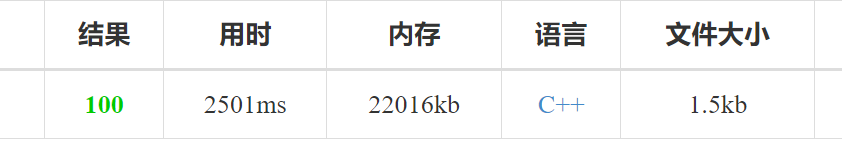
\includegraphics[width=0.8\textwidth]{fft1.png}
	\caption{fft-recursion \label{fig:fft1}}
\end{figure}

\lstinputlisting[language=C++, style=codestyle2]{code07/fft-recursion.cpp}


\subsubsection{FFT的迭代实现}
递归实现的 $FFT$ 效率不高,因为有栈的调用和参数的传递,实际中一般采用迭代实现。

{\heiti 二进制位翻转}

对分治规律的总结:
\begin{figure}[!htbp]
	\centering
	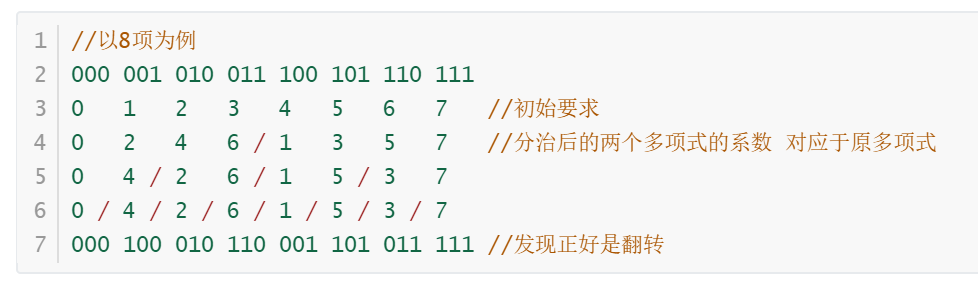
\includegraphics[width=1.0\textwidth]{fft-iter.png}
	\caption{分治的规律 \label{fig:fft-pattern}}
\end{figure}
这为迭代实现提供了理论基础。

{\heiti 蝴蝶操作}

考虑合并两个子问题的过程,假设$A_1(w_{\frac{n}{2}}^k)$ 和$A_2(w_{\frac{n}{2}}^k)$ 分别存放在$a[k]$和$a[\frac{n}{2}+k]$中,$A(w_n^k)$和$A(w_n^{k+\frac{n}{2}})$ 将要存放在$b[k]$和$b[\frac{n}{2}+k]$中,合并的操作可以表示为:
\begin{align*}
b[k]\leftarrow  a[k]+w_n^k*a[\frac{n}{2}+k]  \\
b[k+\frac{n}{2}] \leftarrow a[k]-w_n^k*a[\frac{n}{2}+k]
\end{align*}
考虑加入一个临时变量$t$,使得这个过程可以在原地完成,而不需要数组$b$,	
\begin{align*}
t \leftarrow w_n^k*a[\frac{n}{2}+k]   \\
a[k+\frac{n}{2}] \leftarrow a[k]-t  \\
a[k] \leftarrow a[k]+t
\end{align*}
由于$k$和$k+\frac{n}{2}$ 是对应的,所以不同的$k$之间不会相互影响。

这一过程被称为蝴蝶操作。

\begin{figure}[!htbp]
	\centering
	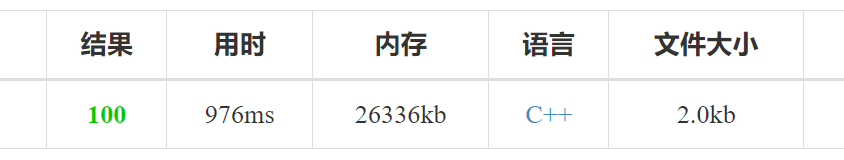
\includegraphics[width=0.8\textwidth]{fft2.png}
	\caption{fft-iteration \label{fig:fft2}}
\end{figure}

\lstinputlisting[language=C++, style=codestyle2]{code07/fft-iteration.cpp}

\subsection{NTT}
由于$FFT$涉及到复数运算,难免有精度问题,在计算一些高精度乘法的时候就有可能由于精度出现错误,这
便让我们考虑是否有在模意义下的方法,这就是{\heiti 快速数论变换}($Fast\ Number-Theoretic\ Transform,\ NTT$)。

首先来看$FFT$中能归并地变换用到了单位根$\omega_n$的什么性质:
\begin{enumerate}
\item $\omega_n^n = 1$;
\item $\omega_n^0\ ,\ \omega_n^1\ ,\ \omega_n^2\ ,\ ...\ ,\ \omega_n^{n-1}$是互不相同的,这样代入计算出来的点值才可以用来还原出多项式的系数;
\item $\omega_n^{k+\frac{n}{2}}=-\omega_n^{k}$,$\ \omega_{2n}^{2k}=\omega_n^k$,这使得问题规模得以减半;
\item $\sum_{i=0}^{n-1}(\omega_n^{j-k})^i = \left\{\begin{matrix}
0,\quad j\neq k\\ 
n,\quad j= k
\end{matrix}\right.$,这使得可以用同样的优化方法加速逆变换。
\end{enumerate}

下面我们要在模意义下寻找满足这些性质的数!

\subsubsection{原根}
由第三章中知一个素数$p$的原根$g$满足$g^0\ ,\ g^1\ ,\ ...\ ,\ g^{p-2}\ (mod\ p)$均不相同。对于一个素数$p$,将其
写成$p=k*2^m + 1$的形式,记$2^m=n$,有$g^{kn}\equiv 1\ (mod\ p)$。我们记$g_n = g^k$,则有$g_n^n\equiv 1\ (mod\ p)$。
由于$g$是$p$的原根,则$g_n^0\ ,\ g_n^1\ ,\ ...\ ,\ g_n^{n-1}$互不相同。

到这里我们发现,在模$p$意义下,$p$的原根$g$的$k$次方$g_n$,具有和单位根$\omega_n$一样的性质!上面已经说明了其具有性质1和性质2。下面说明性质3。

由于$g_n^n\equiv 1\ (mod\ p)$,所以$g_n^{\frac{n}{2}}\equiv 1\ or\ -1\ (mod\ p)$。又由于$g$是原根,则$g_n^{\frac{n}{2}}\equiv -1\ (mod\ p)$。
所以$g_n^{k+\frac{n}{2}}\equiv -g_n^{k}$得证。至于$g_{2n}^{2k}\equiv g_n^k$,只需证$g_n^2\equiv g_{\frac{n}{2}}$。这是比较显然的,因为$k=\frac{p-1}{2^m}$。

对于性质4,证明方法类似,大家可以自行尝试。

因此在$NTT$中,我们可以用原根$g$的$k$次方$g_n$代替$FFT$中的单位根$\omega_{n}$。

\subsubsection{NTT的实现细节}
在$FFT$中,需要预处理$N$项单位根的次幂及其共轭,对应地,$NTT$中也需要。即预处理$g_n^0\ ,\ g_n^1\ ,\ ...\ ,\ g_n^{n-1}$,以及对应的模$p$意义下的逆元。

$NTT$的代码相比$FFT$的代码变动很少。
\begin{note}
\begin{enumerate}
\item 最后逆变换完成后除$n$时,变为乘上$n$关于$p$的逆元即可;
\item $p=k*2^m + 1$中,最大能取到的$2^m$为能处理的结果多项式项数极限。如对于素数$998244353= 119 * 2^{23} + 1$, 最多能处理的$N = 2^{23}$。当$N<2^{23}$时,要将
多余的部分乘到$k$上;(常见的素数及其原根见附录表)
\item 由于实数域上的运算比复数域运算要快,所以$NTT$的运行时间理论上会比$FFT$少;(但由于有取模操作在,所以上述说明是玄学......)
\item 如果一个题目不用取模,使用$NTT$时要注意原本的答案是否会大于等于所选取的模数$p$。
\end{enumerate}
\end{note}

\begin{figure}[!htbp]
	\centering
	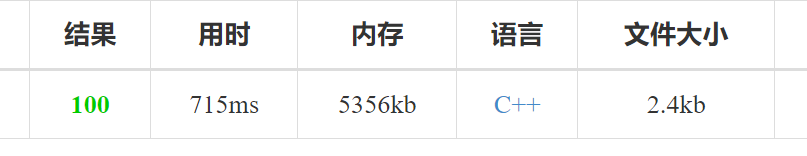
\includegraphics[width=0.8\textwidth]{ntt.png}
	\caption{NTT-iteration \label{fig:ntt}}
\end{figure}

\lstinputlisting[language=C++, style=codestyle2]{code07/NTT.cpp}

\subsubsection{模数任意的解决方案}
$NTT$要求模数写成$p=k*2^m + 1$的形式,但有些题目,要求模数写不成这样的形式,甚至是一个合数。
这样的话,一般选取$s$个常用的素数$p_1\ ,\ p_2\ ,\ ...\ ,\ p_s$,要求满足:
$$
\prod_{i=1}^s p_i > n(m-1)^2
$$
其中$n$是结果多项式的项数,$m$是要求的模数。然后分别在$mod\ p_i$下求解系数,最后使用中国剩余定理将结果合并(一般会使用高精度)。


%\section{多项式}

%\subsection{拉格朗日插值法}

%\subsection{多项式求逆}

%\subsection{多项式取模}

%\subsection{多项式开方}

%\subsection{多项式多点求值}

%\subsection{多项式多点插值}

\vbox{}

\vbox{}

\begin{problemset}
	\item \href{http://poj.org/problem?id=1305}{本原勾股数组 \quad poj 1305}
	\item \href{https://nanti.jisuanke.com/t/41421}{圆上整点/高斯素数 \quad 2019上海网络赛}
	\item \href{https://www.51nod.com/Challenge/Problem.html#problemId=1195}{斐波那契数列循环节 \quad 51nod-1195}
	\item dfs similar \quad 2019icpc亚洲区域赛-南昌站B题
	\item FFT \quad BZOJ 3992 / SDOI2015 序列统计
	\item FFT \quad BZOJ 3771 Triple
	\item \href{https://www.lydsy.com/JudgeOnline/problem.php?id=3527}{BZOJ 3527 \quad FFT}
	\item \href{https://www.luogu.com.cn/problem/P4245}{模板:任意模数NTT}
\end{problemset}


\nocite{*} 

\bibliography{reference}

\appendix

\chapter{常用的表}


\section{梅森素数表}


\section{卡米歇尔数}
1 561

2 1105

3 1729

4 2465

5 2821

6 6601

7 8911

8 10585

9 15841

10 29341

11 41041

12 46657

13 52633

14 62745

15 63973

16 75361

17 101101

18 115921

19 126217

20 162401

21 172081

22 188461

23 252601

24 278545

25 294409

\section{常见的素数及其原根}

\begin{table}[!htbp]
\centering
\caption{常见的素数及其原根 \label{tab:ntt-primes}}
\begin{tabular}{|c|c|c|c|}
\hline
$p=k*2^m + 1$         & $k$   & $m$  & $groot$ \\ \hline
3                   & 1   & 1  & 2     \\ \hline
5                   & 1   & 2  & 2     \\ \hline
17                  & 1   & 4  & 3     \\ \hline
97                  & 3   & 5  & 5     \\ \hline
193                 & 3   & 6  & 5     \\ \hline
257                 & 1   & 8  & 3     \\ \hline
7681                & 15  & 9  & 17    \\ \hline
12289               & 3   & 12 & 11    \\ \hline
40961               & 5   & 13 & 3     \\ \hline
65537               & 1   & 16 & 3     \\ \hline
786433              & 3   & 18 & 10    \\ \hline
5767169             & 11  & 19 & 3     \\ \hline
7340033             & 7   & 20 & 3     \\ \hline
23068673            & 11  & 21 & 3     \\ \hline
104857601           & 25  & 22 & 3     \\ \hline
167772161           & 5   & 25 & 3     \\ \hline
469762049           & 7   & 26 & 3     \\ \hline
{ \color{red}998244353}           & 119 & 23 & 3     \\ \hline
{\color{red}1004535809}          & 479 & 21 & 3     \\ \hline
2013265921          & 15  & 27 & 31    \\ \hline
{\color{red}2281701377}          & 17  & 27 & 3     \\ \hline
3221225473          & 3   & 30 & 5     \\ \hline
75161927681         & 35  & 31 & 3     \\ \hline
77309411329         & 9   & 33 & 7     \\ \hline
206158430209        & 3   & 36 & 22    \\ \hline
2061584302081       & 15  & 37 & 7     \\ \hline
2748779069441       & 5   & 39 & 3     \\ \hline
6597069766657       & 3   & 41 & 5     \\ \hline
39582418599937      & 9   & 42 & 5     \\ \hline
79164837199873      & 9   & 43 & 5     \\ \hline
263882790666241     & 15  & 44 & 7     \\ \hline
1231453023109121    & 35  & 45 & 3     \\ \hline
1337006139375617    & 19  & 46 & 3     \\ \hline
3799912185593857    & 27  & 47 & 5     \\ \hline
4222124650659841    & 15  & 48 & 19    \\ \hline
7881299347898369    & 7   & 50 & 6     \\ \hline
31525197391593473   & 7   & 52 & 3     \\ \hline
180143985094819841  & 5   & 55 & 6     \\ \hline
1945555039024054273 & 27  & 56 & 5     \\ \hline
4179340454199820289 & 29  & 57 & 3     \\ \hline
\end{tabular}
\end{table}
\chapter{最小示例}

\begin{lstlisting}
\documentclass[lang=cn,11pt]{elegantbook}
% title info
\title{Title}
\subtitle{Subtitle is here}
% bio info
\author{Your Name}
\institute{XXX University}
\date{\today}
% extra info
\version{1.00}
\extrainfo{Victory won\rq t come to us unless we go to it. --- M. Moore}
\logo{logo.png}
\cover{cover.jpg}

\begin{document}

\maketitle
\tableofcontents
\mainmatter
\hypersetup{pageanchor=true}
% add preface chapter here if needed
\chapter{Example Chapter Title}
The content of chapter one.

\bibliography{reference}

\end{document}
\end{lstlisting}



\end{document}
